\chapter{Analisi delle mappe di flusso del motore di test}
\raggedbottom
\section{Descrizione del motore di test}
Il motore di test è un motore IPM caratterizzato dai parametri riportati in Tabella \ref{tab:Tabella_parametri_motore}.\\
Dato che il motore possiede due coppie polari, i flussi $\lambda_d$ e $\lambda_q$ presentano una periodicità pari a 90 gradi meccanici. Perciò le mappe di flusso fornite presentano questo range angolare.\\

\begin{table} % Aggiunto [htbp] per il posizionamento
    \centering
    \footnotesize     
    \vspace{0.2cm}

    \renewcommand{\arraystretch}{1.3}
    
    % Definite 4 colonne invece di 3
    \begin{tabular}{
        >{\centering\arraybackslash}m{3 cm}
        >{\centering\arraybackslash}m{2 cm}        
        >{\centering\arraybackslash}m{2 cm} % Colonna aggiunta per pareggiare i conti
        >{\centering\arraybackslash}m{2.5 cm}
        }
        \arrayrulecolor{black}\toprule
        % Sistemata l'intestazione: rimossa la & di troppo
        \textbf{Parametro} & \textbf{Simbolo} & \textbf{Valore} & \textbf{Unità di misura} \\
        \arrayrulecolor{black}\midrule
        \textbf{Coppie polari} & $p$ & 2 & -\\ % p in math mode per il simbolo
        \arrayrulecolor{GRIG}\midrule
        \textbf{Resistenza di statore} &$R_s$ &2.726 & $\Omega$\\
        \arrayrulecolor{GRIG}\midrule
        \textbf{Induttanza di asse D} & $L_d$ & $20.5\cdot10^{-3}$ & $Hz$\\
        \arrayrulecolor{GRIG}\midrule
        \textbf{Induttanza di asse Q} & $L_q$ & 
        $114e\cdot10^{-3}$ & $Hz$\\
        \arrayrulecolor{GRIG}\midrule
        \textbf{Corrente nominale} & $I_n$ & $4.2$ & $A$\\
        \arrayrulecolor{GRIG}\midrule
        \textbf{Corrente nominale} & $I_N$ & $4.2$ & $A$\\
        \arrayrulecolor{GRIG}\bottomrule
        \textbf{Coppia nominale} & $\tau_N$ & $4.5$ & $Nm$\\
        \arrayrulecolor{GRIG}\bottomrule
        \textbf{Flusso magnete permanente} & $\lambda_{mg}$ & $0.22$ & $T$\\    
        \arrayrulecolor{GRIG}\bottomrule
        \textbf{Inerzia meccanica} & $J_m$ & $0.00094$ & $kgm^2$\\
        \arrayrulecolor{GRIG}\bottomrule
        \textbf{Attrito viscoso} & $B_m$ & $0.000155$ & $Nms/rad$\\
        \arrayrulecolor{GRIG}\bottomrule
        \textbf{Coppia di primo distacco} & $T_{ps}$ & $0.065$ & $Nms/rad$\\      
        \arrayrulecolor{black}\bottomrule
    \end{tabular}
    \caption{Parametri fisici del motore.}
    \label{tab:Tabella_parametri_motore}
\end{table}


\begin{table}[htbp] % Aggiunto [htbp] per il posizionamento
    \centering
    \footnotesize     
    \vspace{0.2cm}

    \renewcommand{\arraystretch}{1.3}
    
    % Definite 4 colonne invece di 3
    \begin{tabular}{
        >{\centering\arraybackslash}m{3 cm}
        >{\centering\arraybackslash}m{2 cm}        
        >{\centering\arraybackslash}m{2 cm} % Colonna aggiunta per pareggiare i conti
        >{\centering\arraybackslash}m{2.5 cm}
        }
        \arrayrulecolor{black}\toprule
        % Sistemata l'intestazione: rimossa la & di troppo
        \textbf{Parametro} &  \textbf{Valore} & \textbf{Unità di misura} \\
        \arrayrulecolor{black}\midrule
        \textbf{Risoluzione di posizione} & $2\pi/2^{16}$ & $rad$\\ % p in math mode per il simbolo
        \arrayrulecolor{GRIG}\midrule
        \textbf{Risoluzione di corrente} &0.001 & $A$\\
        \arrayrulecolor{GRIG}\midrule
        \textbf{Risoluzione di tensione} & 0.01 & $V$\\
        \arrayrulecolor{GRIG}\midrule
        \textbf{Frequenza di campionamento} & 10 & $KHz$\\
        \arrayrulecolor{black}\bottomrule
    \end{tabular}
    \caption{Parametri del sistema di misura.}
    \label{tab:Tabella_parametri_misura}
\end{table}

\section{Confronto dell'andamento del flusso con la velocità del rotore}
Per valutare l'effetto della velocità sul flusso magnetico concatenato, si sono confrontati gli andamenti del flusso all'aumentare della velocità.\\
Si può notare come, anche in questo caso, l'influenza della dipendenza dalla posizione nell'andamento due flussi sia simile. 

\begin{figure}
\centering
    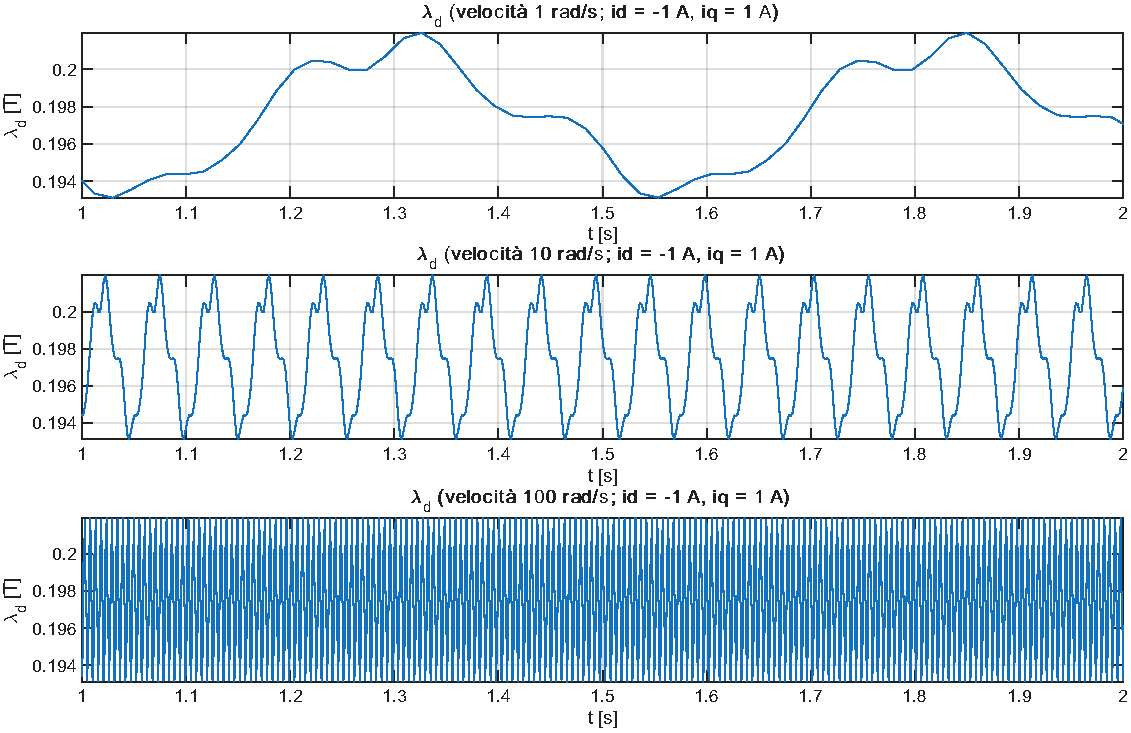
\includegraphics[height=7.5 cm]{immagini/flusso_concatenato/iq=m1/flusso_D_vs_velocità_iq_1.pdf}
    \caption{Andamento del flusso D al variare della velocità ($i_d$ = $i_q$ = -1 A).}
    \label{fig:flusso_D_vs_velocità_1}
\end{figure}

\begin{figure}
\centering
    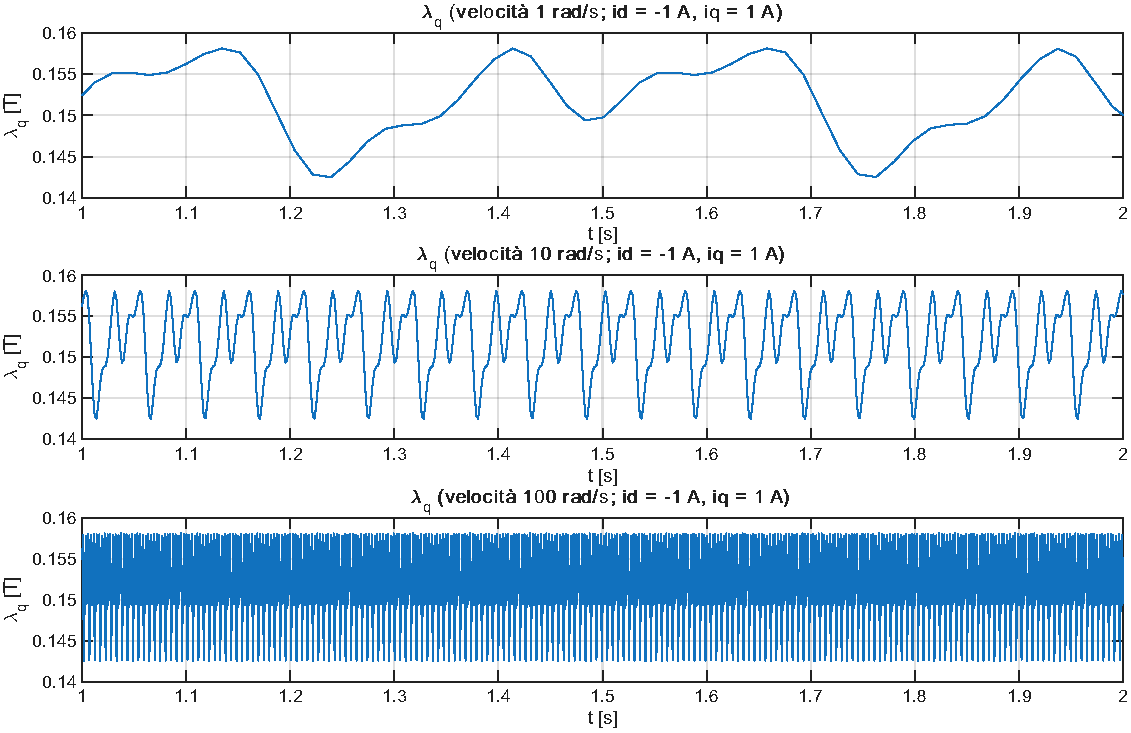
\includegraphics[height=7.5 cm]{immagini/flusso_concatenato/iq=m1/flusso_Q_vs_velocità_iq_1.pdf}
    \caption{Andamento del flusso Q al variare della velocità ($i_d$ = -1 A, $i_q$ = 1 A).}
    \label{fig:flusso_Q_vs_velocità_1}
\end{figure}







\section{Analisi delle armoniche del disturbo}
Si può notare come all'aumentare della velocità aumenti la frequenza dell'armonica principale del disturbo, mentre l'ampiezza rimane pressoché uguale. Non si riscontrano significative differenze tra le armoniche dei due flussi. 
Dall'analisi delle mappe di flusso si osserva come l'andamento del flusso si ripeta 3 volte in 90° meccanici, quindi 12 volte in una rotazione completa. Ciò permette di individuare dove è situata la fondamentale del disturbo sul flusso al variare della velocità meccanica, $\omega_m$ (1 rad/s):
\begin{equation}
    f_0=\frac{\omega_m\cdot 12}{2\pi} = 1.910 \ Hz
\end{equation}

 Conoscere questo dato diviene utile nel caso dell'aggiunta di un filtro passa alto per la rimozione del rumore a bassa frequenza; ciò permette di eliminare i disturbi senza attenuare o sfasare la prima armonica.


\begin{figure}
\centering
    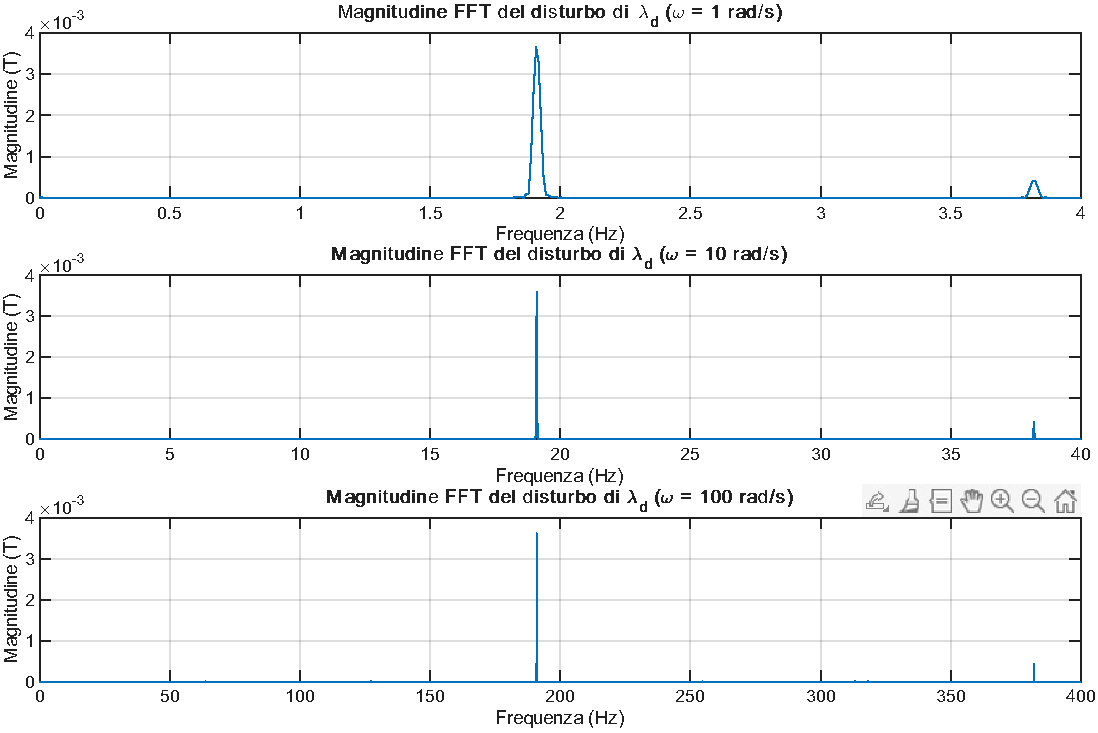
\includegraphics[height=7.5 cm]{immagini/flusso_concatenato/iq=m1/FFT_flusso_D_iq_1.pdf}
    \caption{FFT del flusso D al variare della velocità ($i_d$ = -1 A, $i_q$ = 1 A).}
    \label{fig:FFT_flusso_D_1}
\end{figure}

\begin{table}
    \centering
        
    \footnotesize
    
    \textbf{Analisi sul flusso $\lambda_d$}       
    
    \vspace{0.2cm}

    \renewcommand{\arraystretch}{1.3}
    
    \begin{tabular}{
        >{\centering\arraybackslash}m{3 cm}
        >{\centering\arraybackslash}m{2 cm}        
        >{\centering\arraybackslash}m{2.5 cm}
        }
\arrayrulecolor{black}\toprule
        \textbf{Velocità meccanica } &$\mathbf{Ampiezza}$ &$\mathbf{Frequenza}$ \\
       \text{[\,rad/s\,]} &\text{[\,V\,]} &\text{[\,Hz\,]} \\
            \arrayrulecolor{black}\midrule
            \textbf{1} & 0.00368 & 1.907 \\
            \arrayrulecolor{GRIG}\midrule
            \textbf{10}      & 0.00362 & 19.102 \\
            \arrayrulecolor{GRIG}\midrule
            \textbf{100}      & 0.00365 & 190.983 \\
        \arrayrulecolor{black}\bottomrule
    \end{tabular}
    \caption{Analisi sul flusso $\lambda_d$ con $i_d\ = \ -1\ A$ e $i_q\ = \ 1\ A$.}
    \label{tab:valore_forme_d'onda_flusso_D}   
\end{table}

Nel caso della FFT di $\lambda_q$ (Figura \ref{fig:FFT_flusso_Q_1}) si può notare come l'armonica con ampiezza maggiore sia collocata a una frequenza più alta rispetto a $\lambda_d$ (Figura \ref{fig:FFT_flusso_D_1}). I risultati numerici della FFT sono riportati in Figura \ref{tab:valore_forme_d'onda_flusso_D} e \ref{tab:valore_forme_d'onda_flusso_Q}.\\
Le forme d'onda del flusso vengono riportate nelle Figure \ref{fig:flusso_D_vs_velocità_1} e \ref{fig:flusso_Q_vs_velocità_1}. Ciò è dovuto alla forma particolare del segnale periodico, che presenta due picchi e non uno unico, come nel caso di $\lambda_d$. 





\begin{figure}
\centering
    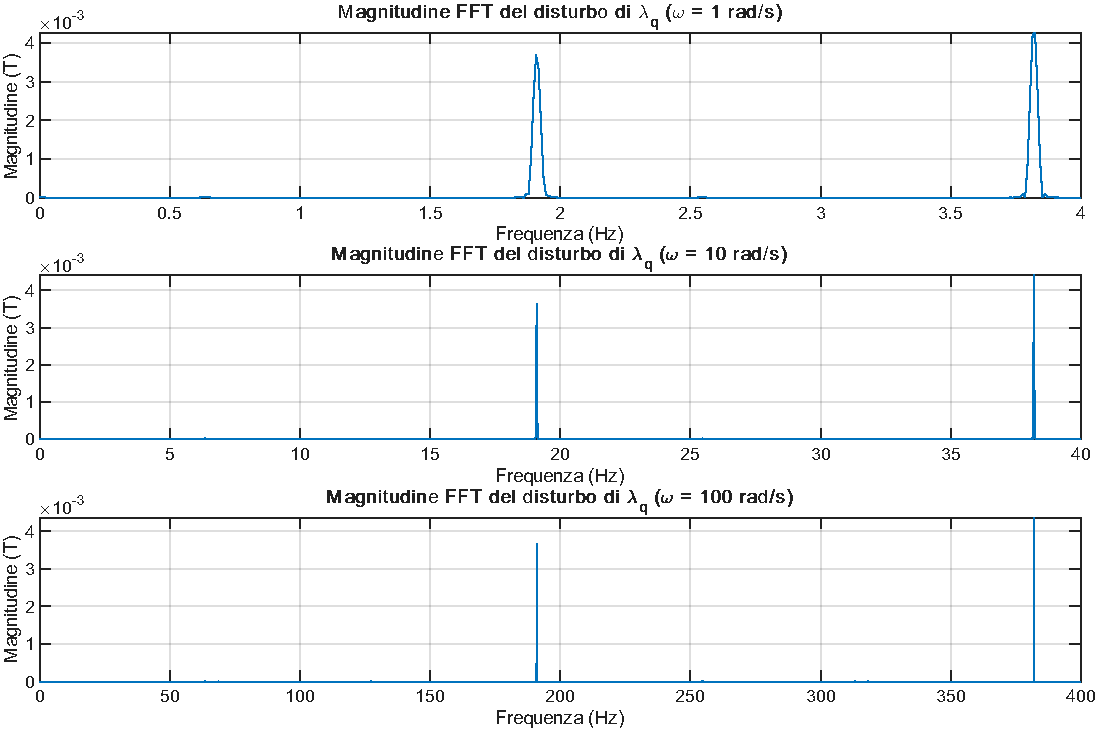
\includegraphics[height=7.5 cm]{immagini/flusso_concatenato/iq=m1/FFT_flusso_Q_iq_1.pdf}
    \caption{FFT del flusso Q al variare della velocità ($i_d$ = -1 A, $i_q$ = 1 A).}
    \label{fig:FFT_flusso_Q_1}
\end{figure}

\begin{table}
    \centering
        
    \footnotesize
    
    \textbf{Analisi sul flusso $\lambda_q$}       
    
    \vspace{0.2cm}

    \renewcommand{\arraystretch}{1.3}
    
    \begin{tabular}{
        >{\centering\arraybackslash}m{3 cm}
        >{\centering\arraybackslash}m{2 cm}        
        >{\centering\arraybackslash}m{2.5 cm}
        }
\arrayrulecolor{black}\toprule
        \textbf{Velocità meccanica } &$\mathbf{Ampiezza}$ &$\mathbf{Frequenza}$ \\
       \text{[\,rad/s\,]} &\text{[\,V\,]} &\text{[\,Hz\,]} \\
            \arrayrulecolor{black}\midrule
            \textbf{1} & 0.0045 & 3.815 \\
            \arrayrulecolor{GRIG}\midrule
            \textbf{10}      & 0.0046 & 38.193 \\
            \arrayrulecolor{GRIG}\midrule
            \textbf{100}      & 0.0047 & 381.97 \\
        \arrayrulecolor{black}\bottomrule
    \end{tabular}
    \caption{Analisi sul flusso $\lambda_q$ con $i_d\ = \ -1\ A$ e $i_q\ = \ 1\ A$.}
    \label{tab:valore_forme_d'onda_flusso_Q}   
\end{table}


\section{Valutazioni sull'impatto della posizione e corrente sul flusso}
Per valutare l'effettiva influenza delle correnti e della posizione meccanica, sono stati analizzati diversi grafici.\\
L'obiettivo dell'analisi è comprendere più a fondo la natura della mappa magnetica del motore e verificare l'impatto della dipendenza dalla posizione.




\subsection{Analisi del flusso $\lambda_{dq}$ espresso in funzione delle correnti.}
Si può notare anche come l'andamento del flusso $\lambda_d$ rimanga invariato invertendo il segno della corrente $i_q$ (Figure \ref{fig:Flusso_D_vs_Id_thetaVar} e \ref{fig:Flusso_D_vs_Id_thetaVar_iq_1}).\\
Fissando la corrente $i_q$, si può osservare come i flussi $\lambda_d$ e $\lambda_q$ abbiano un andamento monotono crescente (Figure \ref{fig:Flusso_D_vs_Id_thetaVar_iq_1} e \ref{fig:Flusso_Q_vs_Id_thetaVar_iq_1}).\\
Tale andamento crescente si riscontra anche con il flusso $\lambda_q$ fissando la corrente $i_d$ (Figura \ref{fig:Flusso_D_vs_Iq_thetaVar}). Al contrario, il flusso $\lambda_d$ con $i_d$ fissa non presenta questa tendenza.\\
Nel caso del cross-coupling si riscontra un maggiore effetto della variazione della posizione (Figure \ref{fig:Flusso_D_vs_Id_thetaVar_iq_1}, \ref{fig:Flusso_D_vs_Iq_thetaVar}  e \ref{fig:Flusso_Q_vs_Id_thetaVar}). Nell'accoppiamento diretto invece l'effetto è meno significativo e quasi ininfluente nel caso della Figura \ref{fig:Flusso_Q_vs_Iq_thetaVar}. 


\begin{figure}
\centering
    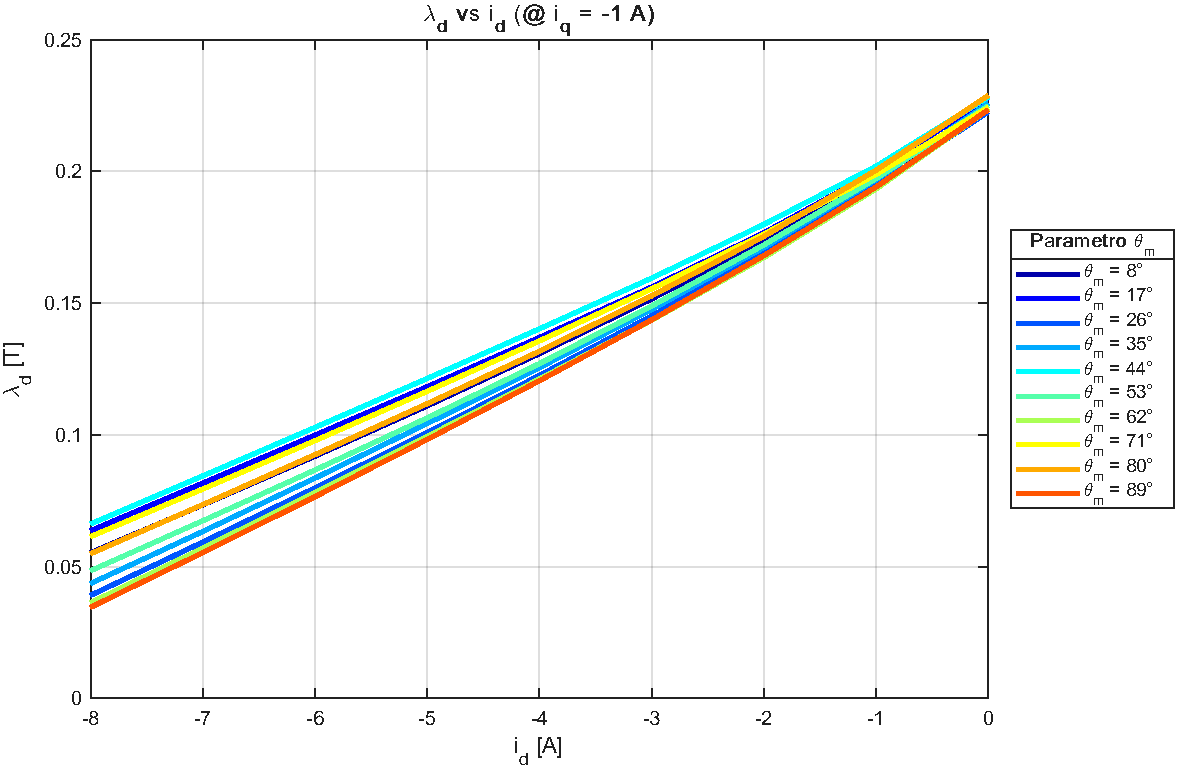
\includegraphics[height=7.5 cm]{immagini/flusso_concatenato/Flusso_D_vs_Id_thetaVar.pdf}
    \caption{Andamento del flusso D in funzione di $i_d$ a seconda della posizione @ $i_q$ = -1 A.}
    \label{fig:Flusso_D_vs_Id_thetaVar}
\end{figure}

\begin{figure}
\centering
    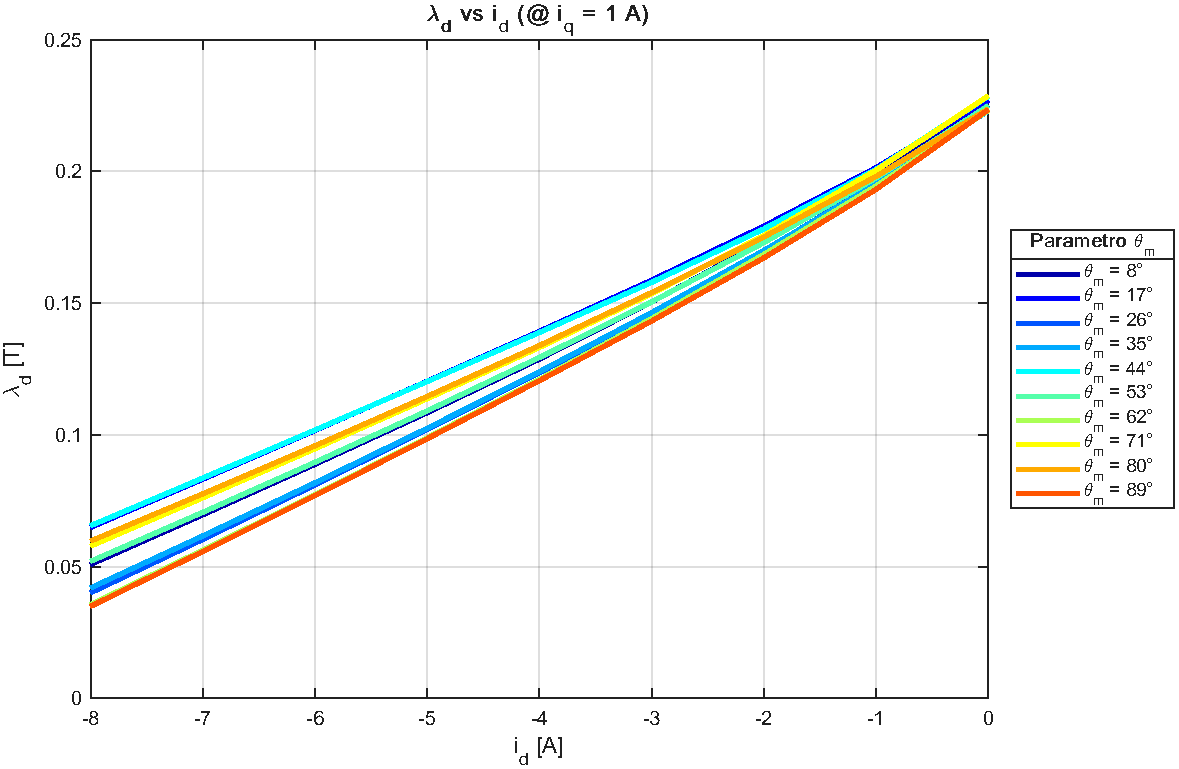
\includegraphics[height=7.5 cm]{immagini/flusso_concatenato/iq=m1/Flusso_D_vs_Id_thetaVar_iq_1.pdf}
    \caption{Andamento del flusso D in funzione di $i_d$ a seconda della posizione @ $i_q$ = 1 A.}
    \label{fig:Flusso_D_vs_Id_thetaVar_iq_1}
\end{figure}

\begin{figure}
\centering
    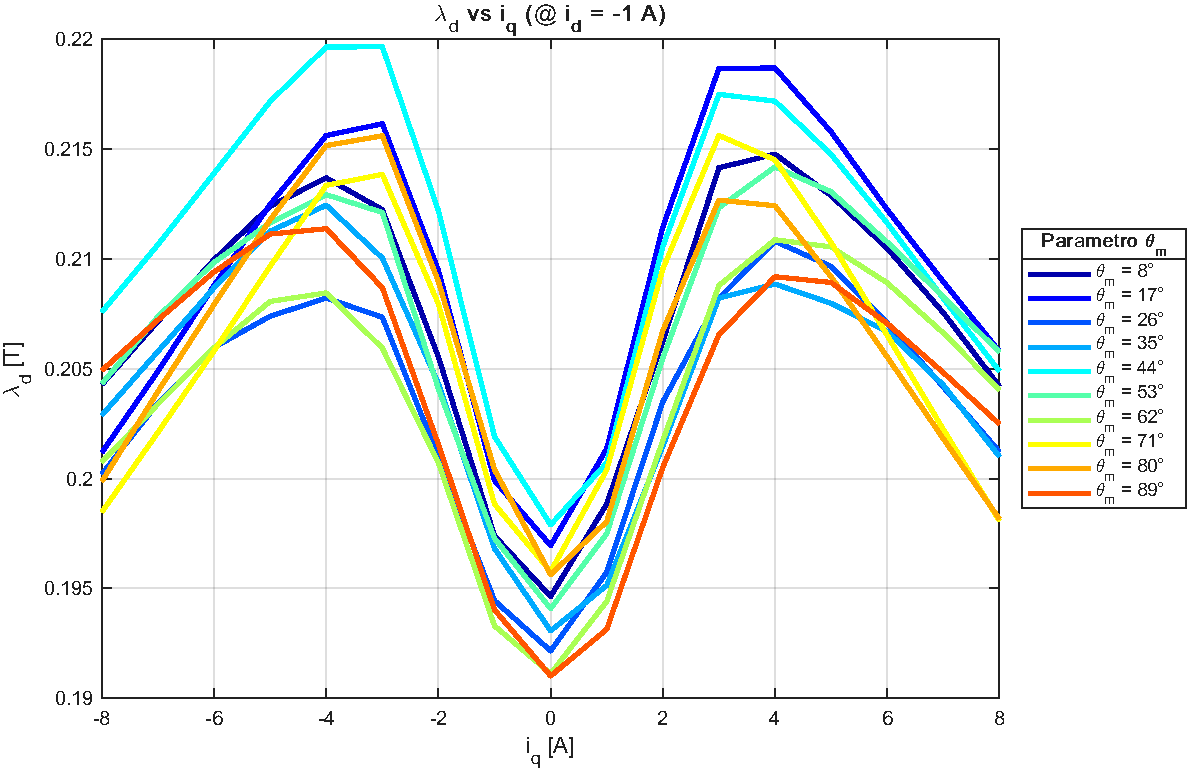
\includegraphics[height=7.5 cm]{immagini/flusso_concatenato/Flusso_D_vs_Iq_thetaVar.pdf}
    \caption{Andamento del flusso D in funzione di $i_q$ a seconda della posizione @ $i_d$ = -1 A.}
    \label{fig:Flusso_D_vs_Iq_thetaVar}
\end{figure}




\begin{figure}
\centering
    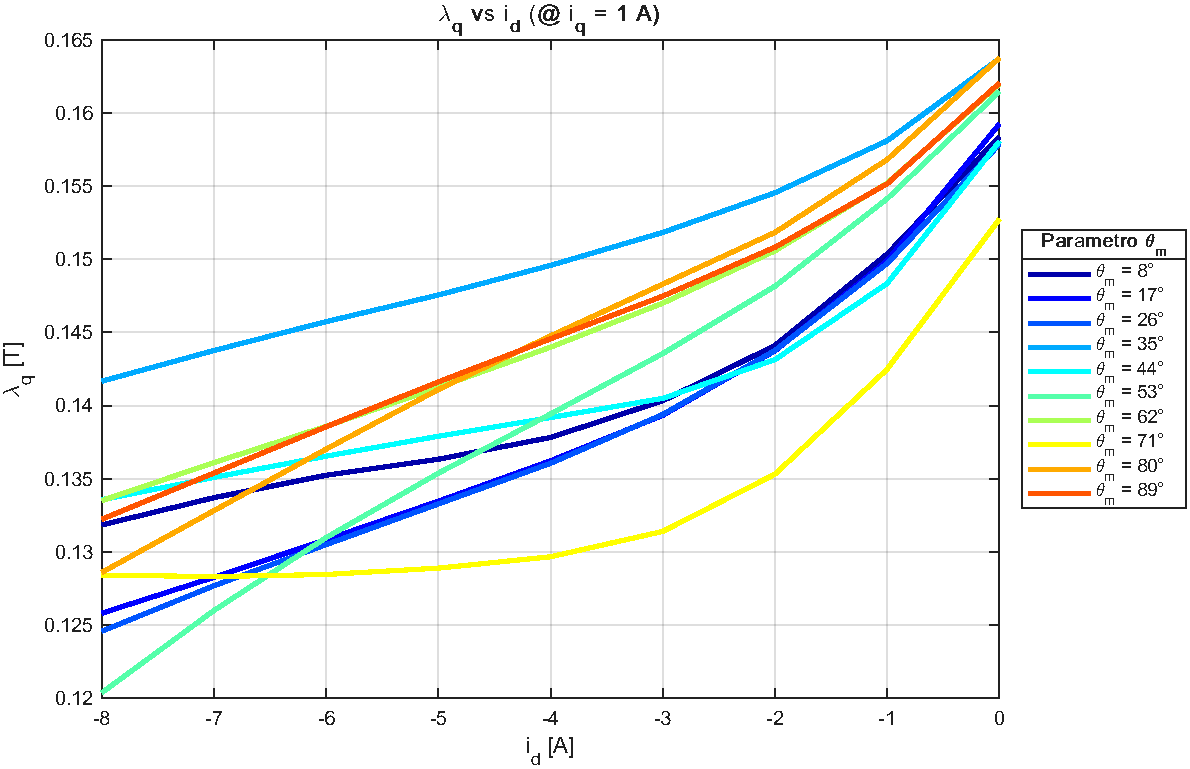
\includegraphics[height=7.5 cm]{immagini/flusso_concatenato/Flusso_Q_vs_Id_thetaVar.pdf}
    \caption{Andamento del flusso Q in funzione di $i_d$ a seconda della posizione @ $i_q$ = -1 A.}
    \label{fig:Flusso_Q_vs_Id_thetaVar}
\end{figure}


\begin{figure}
\centering
    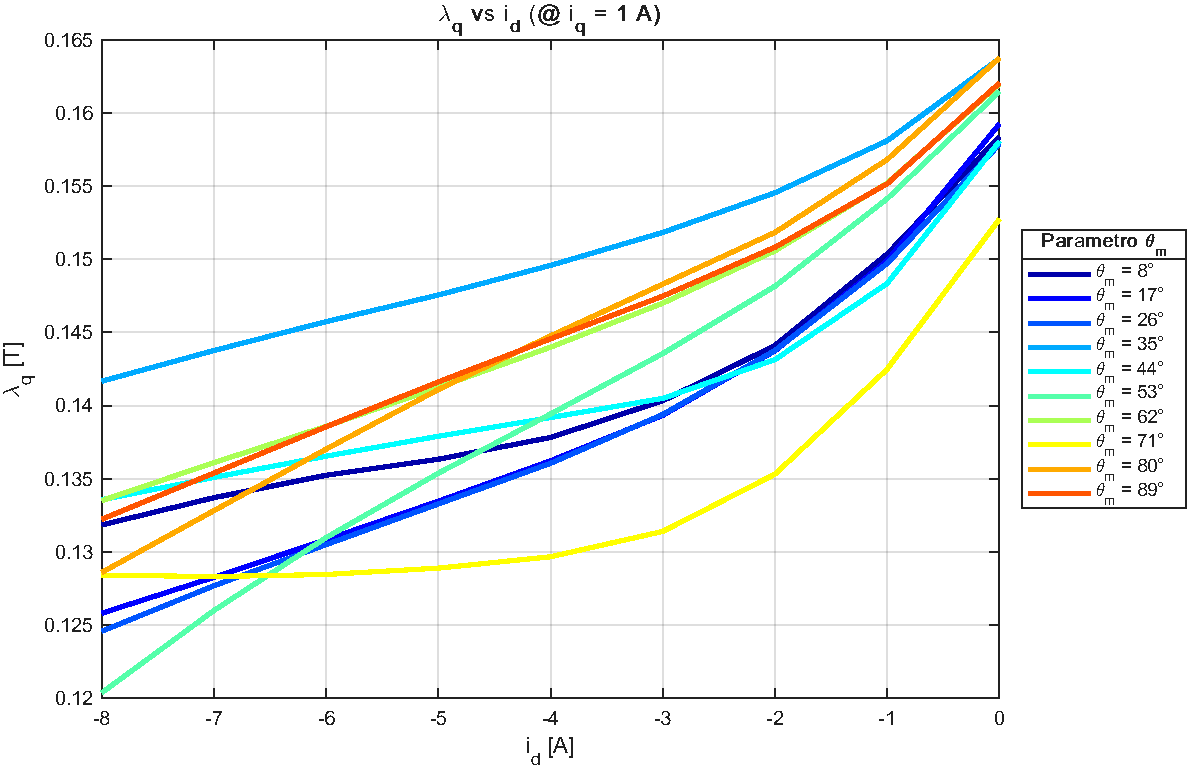
\includegraphics[height=7.5 cm]{immagini/flusso_concatenato/iq=m1/Flusso_Q_vs_Id_thetaVar_iq_1.pdf}
    \caption{Andamento del flusso Q in funzione di $i_d$ a seconda della posizione @ $i_q$ = 1 A.}
    \label{fig:Flusso_Q_vs_Id_thetaVar_iq_1}
\end{figure}

\begin{figure}
\centering
    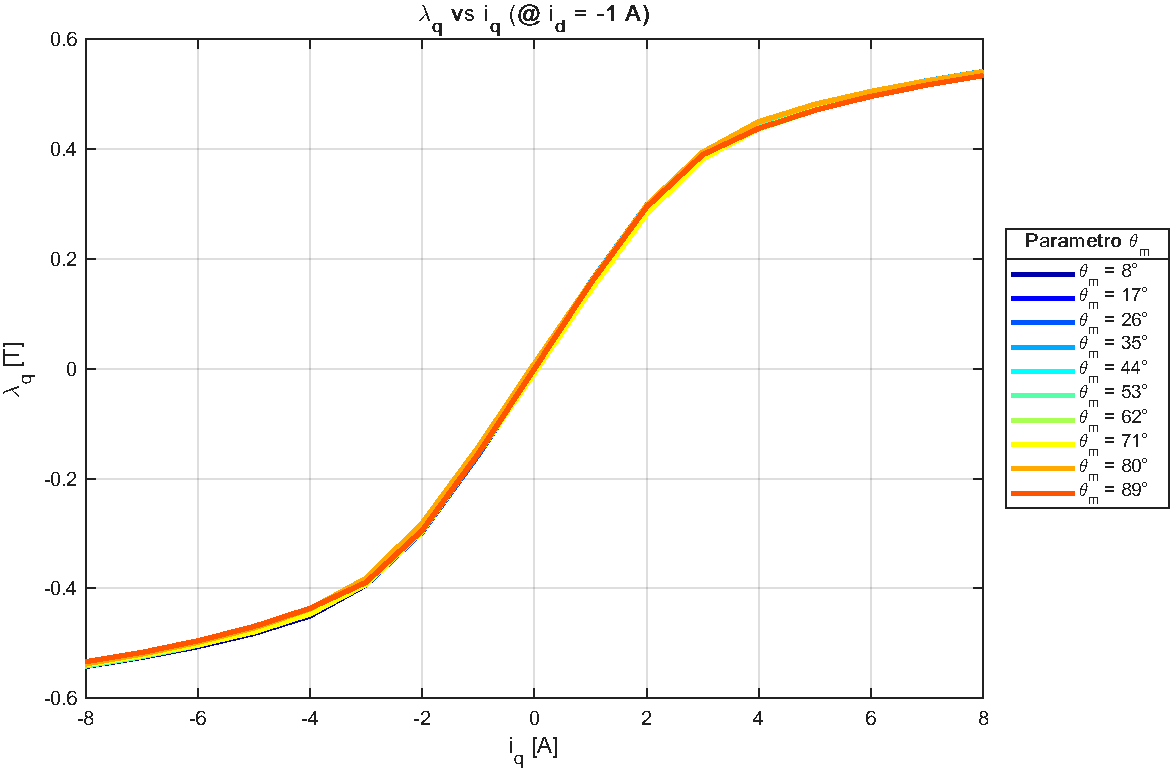
\includegraphics[height=7.5 cm]{immagini/flusso_concatenato/Flusso_Q_vs_Iq_thetaVar.pdf}
    \caption{Andamento del flusso Q in funzione di $i_q$ a seconda della posizione @ $i_d$ = -1 A.}
    \label{fig:Flusso_Q_vs_Iq_thetaVar}
\end{figure}

\subsection{Analisi del flusso $\lambda_{dq}$ espresso in funzione della posizione.}
Successivamente sono riportati i grafici del flusso in funzione della posizione.
Si può notare come l'impatto della posizione sul valore del flusso dipenda dall'intensità della corrente.\\ L'inversione di $i_q$ non influenza il flusso $\lambda_d$, rispetto al quale presenta un comportamento simmetrico (Figure  \ref{fig:Flusso_D_vs_theta_IdVar} e \ref{fig:Flusso_D_vs_theta_IdVar_iq_1}).\\
Al contrario, il legame tra la corrente $i_q$ e il flusso $\lambda_q$ è di tipo antisimmetrico: invertendo il segno della corrente, si inverte il segno del flusso (Figure  \ref{fig:Flusso_Q_vs_theta_IdVar} e \ref{fig:Flusso_Q_vs_theta_IdVar_iq_1}).\\
Nelle Figure \ref{fig:Flusso_D_vs_theta_IdVar} e \ref{fig:Flusso_D_vs_theta_IdVar_iq_1} si può anche notare come l'ampiezza del flusso magnetico $\lambda_d$ e il valore medio tenda ad incrementare all'aumentare del parametro di corrente $i_d$.
Nella Figura \ref{fig:Flusso_D_vs_theta_IqVar2}, si osserva come l'ampiezza picco-picco del disturbo aumenti all'aumentare della corrente $i_d$. Anche in questo caso è confermato che il disturbo influenza maggiormente il cross-coupling.\\
Nella Figura \ref{fig:Flusso_Q_vs_theta_IdVar}, si osserva come l'ampiezza picco-picco del disturbo sia ridotta e rimanga pressochè inalterata al variare della corrente $i_q$.
Confrontando la Figura \ref{fig:Flusso_Q_vs_theta_IdVar} e la Figura \ref{fig:Flusso_Q_vs_theta_IdVar_iq_1} si può notare l'antisimmetricità del flusso $\lambda_q$ rispetto alla corrente $i_q$.\\
In Figura \ref{fig:Flusso_Q_vs_theta_IqVar} viene ripoertato l'andamento del flusso, fissando la corrente $i_d$.

\begin{figure}
\centering
    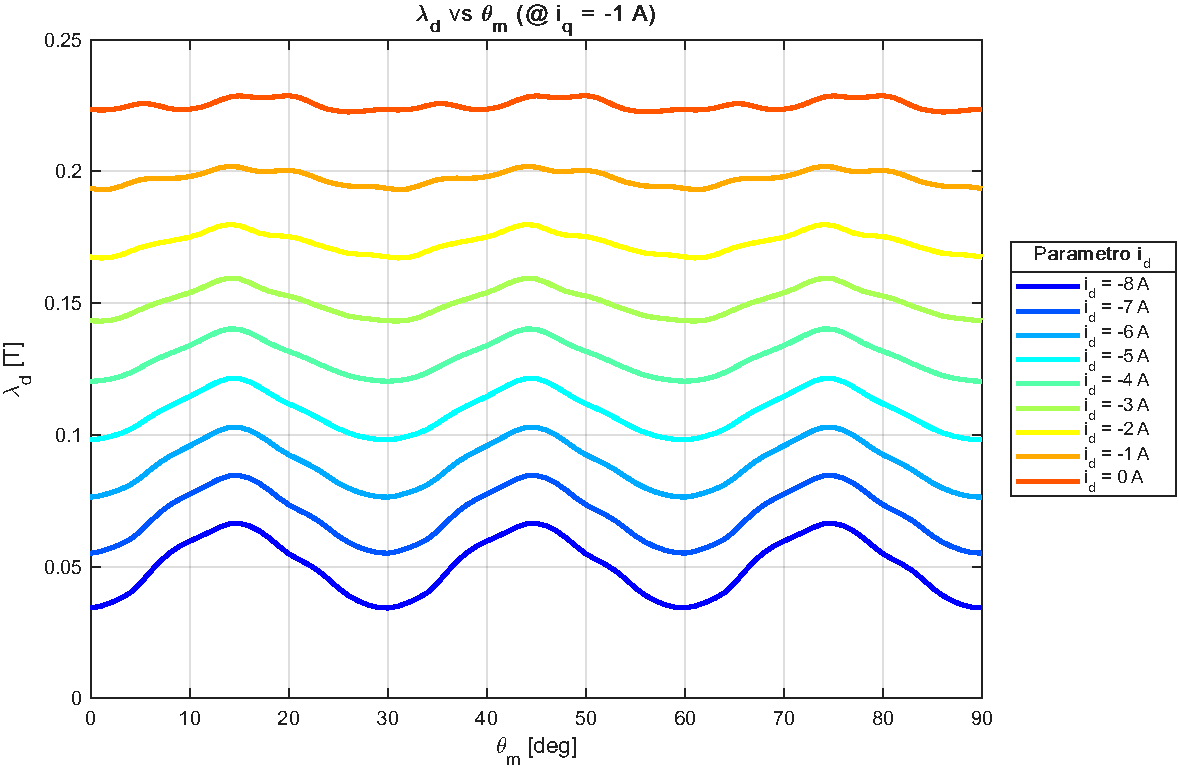
\includegraphics[height=7.5 cm]{immagini/flusso_concatenato/Flusso_D_vs_theta_IdVar.pdf}
    \caption{Andamento del flusso D in funzione di $\theta_m$ a seconda della posizione @ $i_q$ = -1 A. Massima ampiezza picco-picco = 0.0375 T. Massima deviazione standard (disturbo) = 0.0132 T.}
    \label{fig:Flusso_D_vs_theta_IdVar}
\end{figure}



\begin{figure}
\centering
    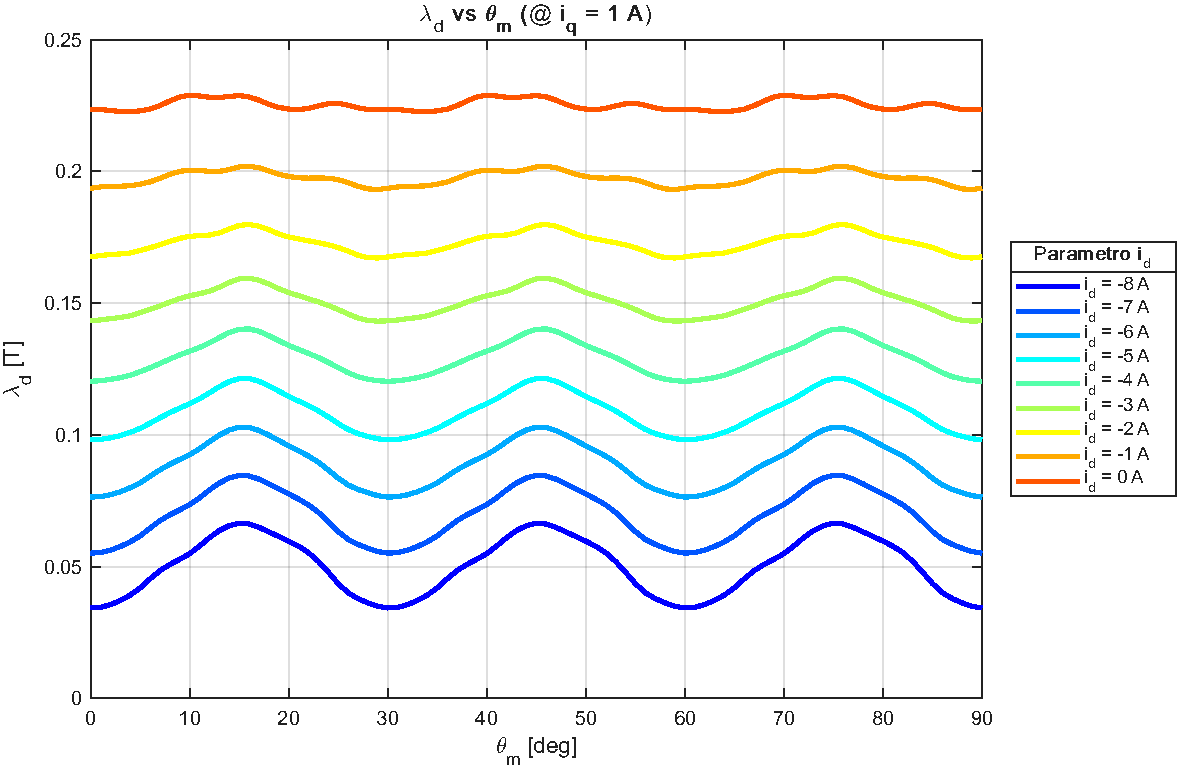
\includegraphics[height=7.5 cm]{immagini/flusso_concatenato/iq=m1/Flusso_D_vs_theta_IdVar_iq_1.pdf}
    \caption{Andamento del flusso D in funzione di $\theta_m$ a seconda della posizione @ $i_q$ = 1 A. Massima ampiezza picco-picco = 0.0375 T. Massima deviazione standard (disturbo) = 0.0132 T.}
    \label{fig:Flusso_D_vs_theta_IdVar_iq_1}
\end{figure}

\begin{figure}
\centering
    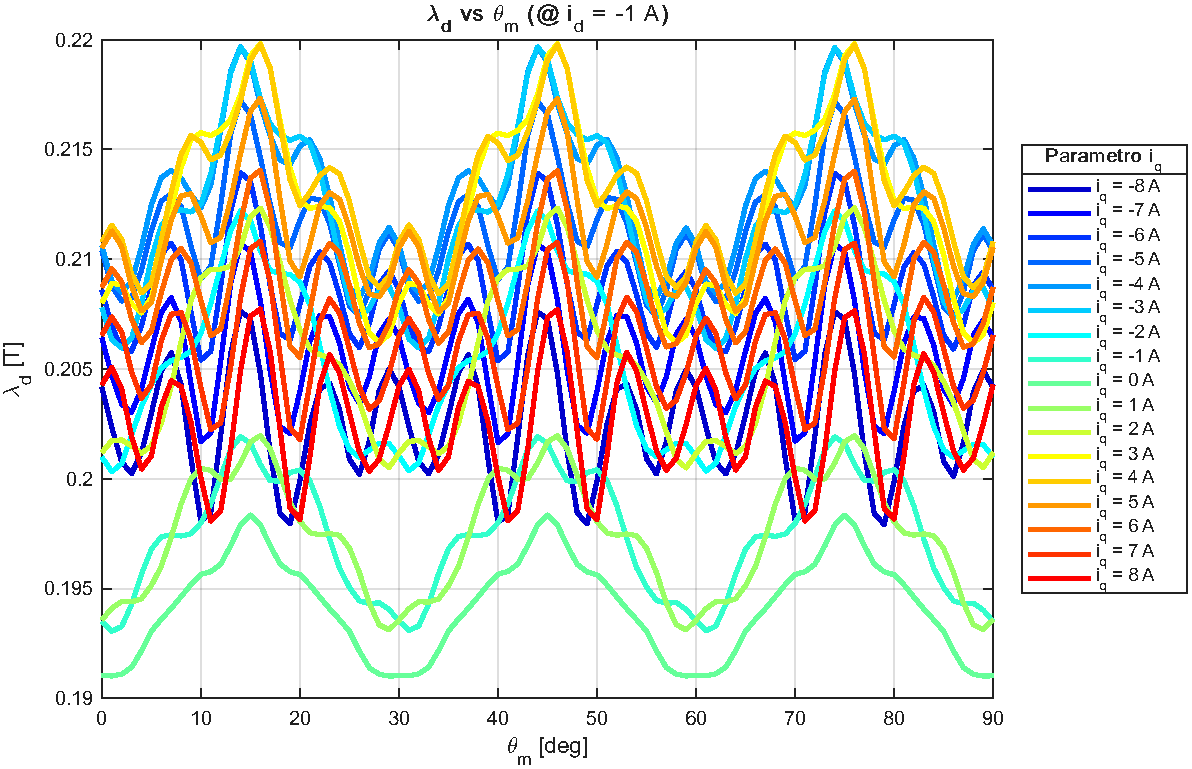
\includegraphics[height=7.5 cm]{immagini/flusso_concatenato/Flusso_D_vs_theta_IqVar.pdf}
    \caption{Andamento del flusso D in funzione di $\theta_m$ a seconda della posizione @ $i_d$ = -1 A. Massima ampiezza picco-picco = 0.0143 T. Massima deviazione standard (disturbo) = 0.0041 T. }
    \label{fig:Flusso_D_vs_theta_IqVar2}
\end{figure}



\begin{figure}
\centering
    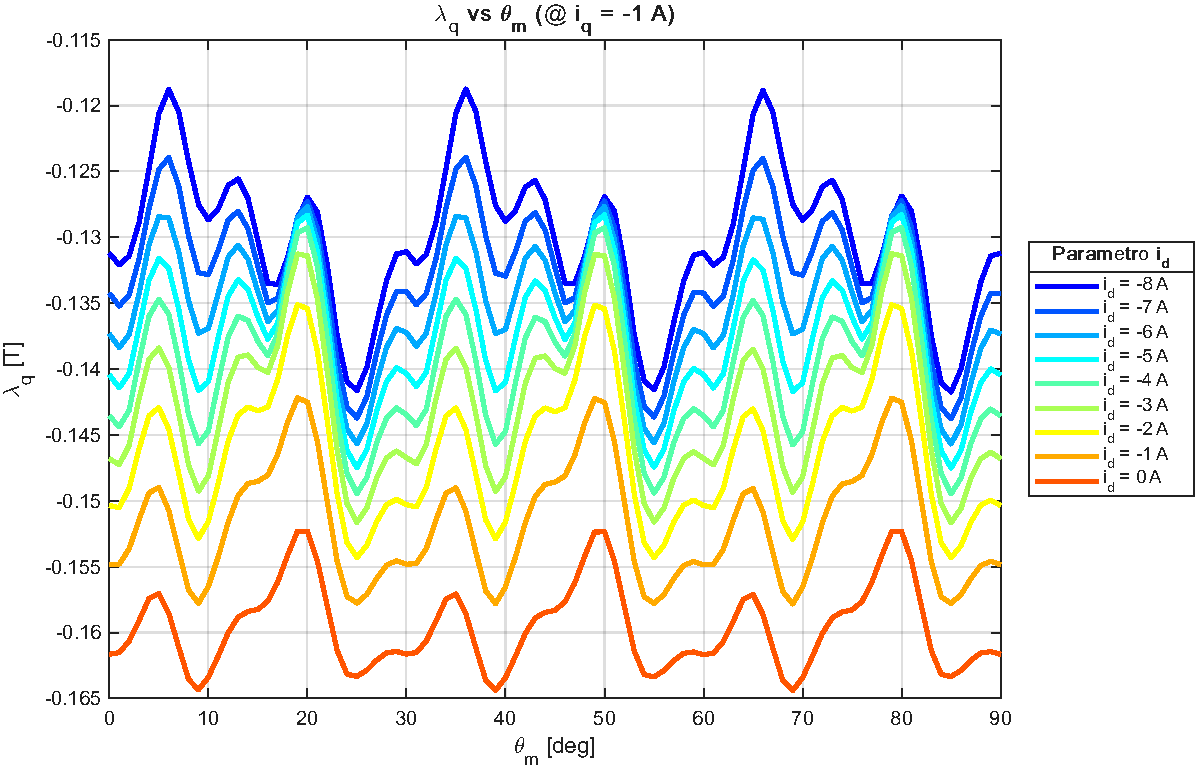
\includegraphics[height=7.5 cm]{immagini/flusso_concatenato/Flusso_Q_vs_theta_IdVar.pdf}
    \caption{Andamento del flusso Q in funzione di $\theta_m$ a seconda della posizione @ $i_q$ = -1 A. Massima ampiezza picco-picco = 0.0345 T. Massima deviazione standard (disturbo) = 0.0087 T.}
    \label{fig:Flusso_Q_vs_theta_IdVar}
\end{figure}


\begin{figure}
\centering
    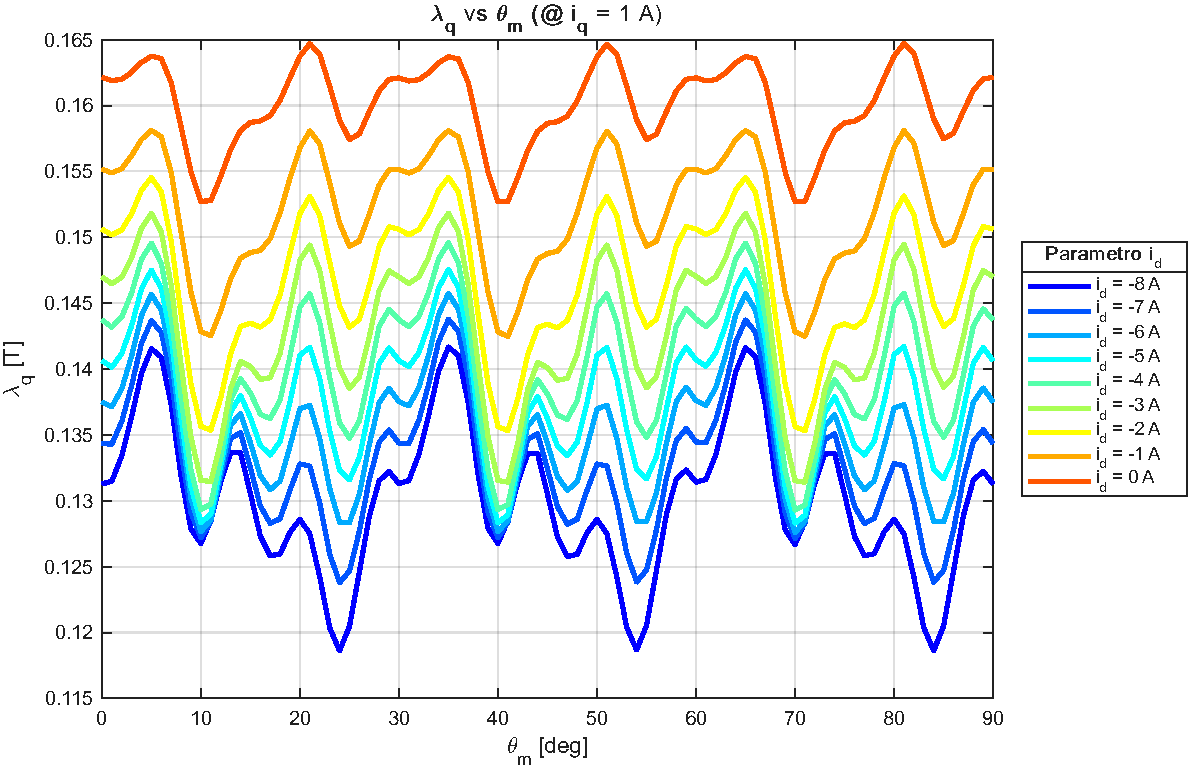
\includegraphics[height=7.5 cm]{immagini/flusso_concatenato/iq=m1/Flusso_Q_vs_theta_IdVar_iq_1.pdf}
    \caption{Andamento del flusso Q in funzione di $\theta_m$ a seconda della posizione @ $i_q$ = 1 A. Massima ampiezza picco-picco = 0.0344 T. Massima deviazione standard (disturbo) = 0.0087 T.}
    \label{fig:Flusso_Q_vs_theta_IdVar_iq_1}
\end{figure}




\begin{figure}
\centering
    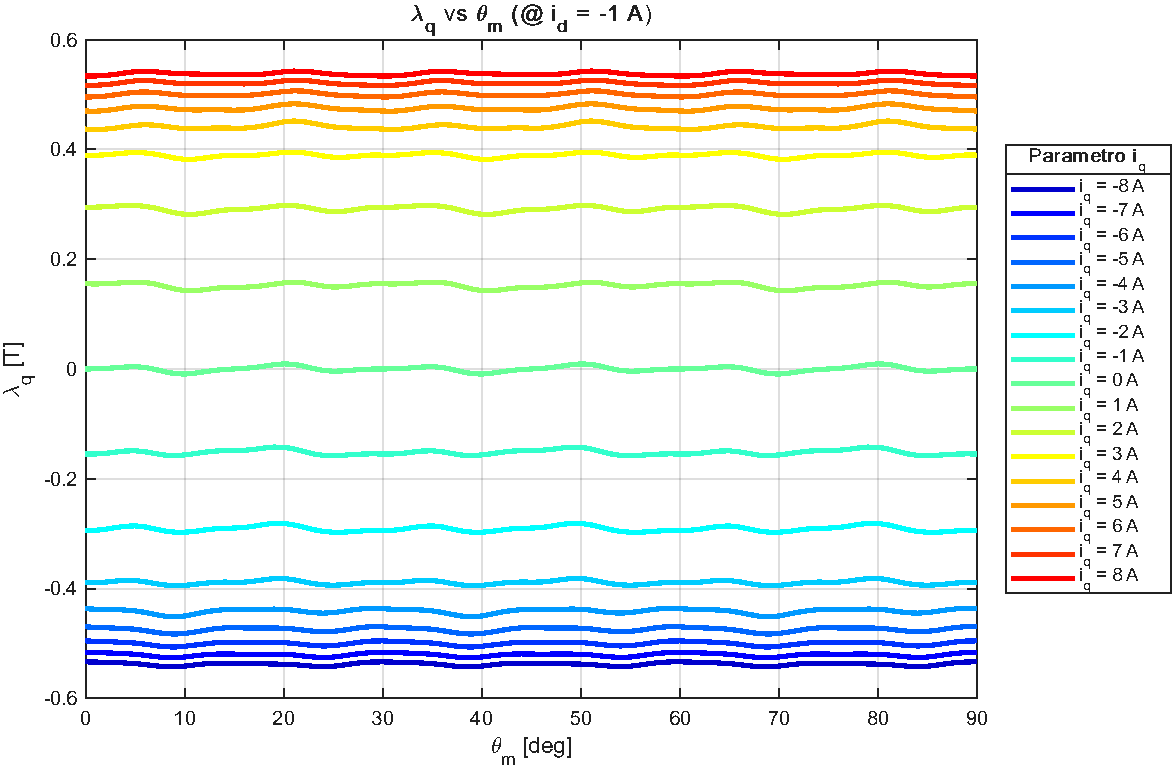
\includegraphics[height=7.5 cm]{immagini/flusso_concatenato/Flusso_Q_vs_theta_IqVar.pdf}
    \caption{Andamento del flusso Q in funzione di $\theta_m$ a seconda della posizione @ $i_d$ = -1 A. Massima ampiezza picco-picco = 0.0199 T. Massima deviazione standard (disturbo) = 0.0051 T.}
    \label{fig:Flusso_Q_vs_theta_IqVar}
\end{figure}



\subsection{Analisi della fcem}
Si riporta poi l'andamento della fcem al variare della velocità meccanica. Si può notare come all'aumentare della velocità aumenti l'ampiezza del disturbo sulla fcem e la frequenza del segnale (Figure \ref{fig:fcem_D_vs_velocità} e \ref{fig:fcem_Q_vs_velocità}). Questo andamento è confermato anche dai dati riportati nelle Tabelle \ref{tab:valore_forme_d'onda_fcem_D} e \ref{tab:valore_forme_d'onda_fcem_Q}. Questo è un comportamento atteso, dato il legame che lega la velocità di rotazione alla fcem:
\begin{equation}
 e_{dq}=\omega_{e}\cdot \lambda_{dq}
\end{equation}
\begin{figure}
\centering
    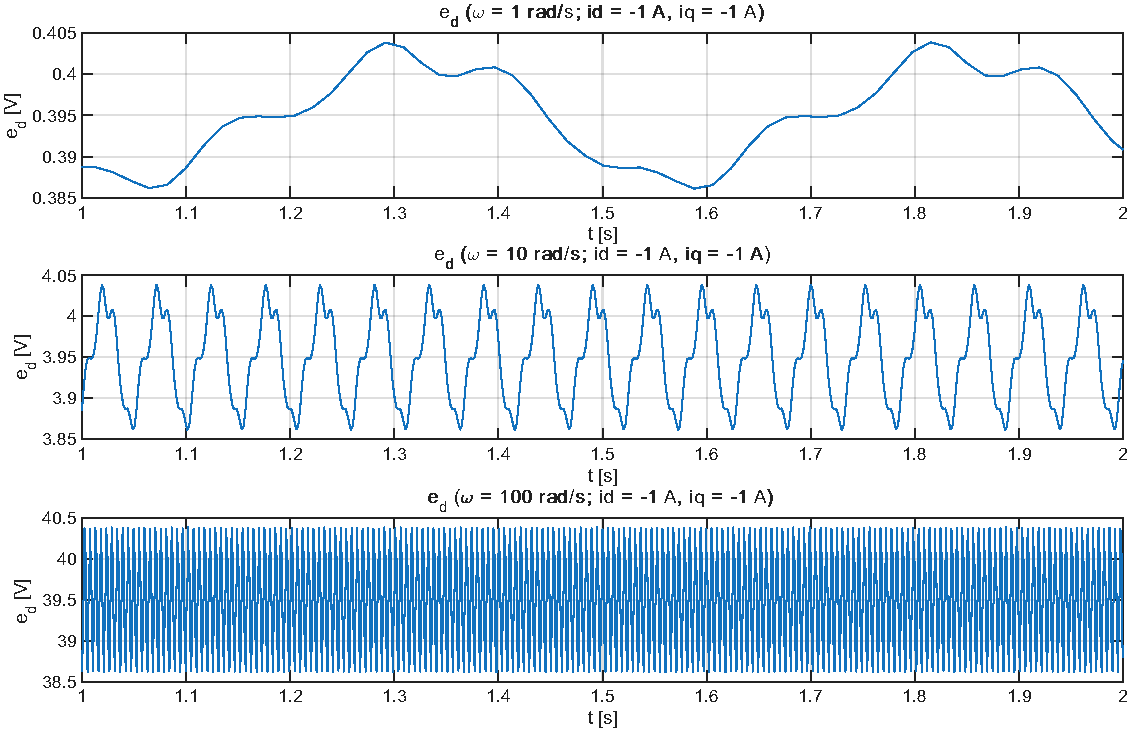
\includegraphics[height=7.5 cm]{immagini/fcem/fcem_D_vs_velocità.pdf}
    \caption{Andamento della tensione fcem D al variare della velocità ($i_d$ = -1 A, $i_q$ = -1 A).}
    \label{fig:fcem_D_vs_velocità}
\end{figure}



\begin{figure}
\centering
    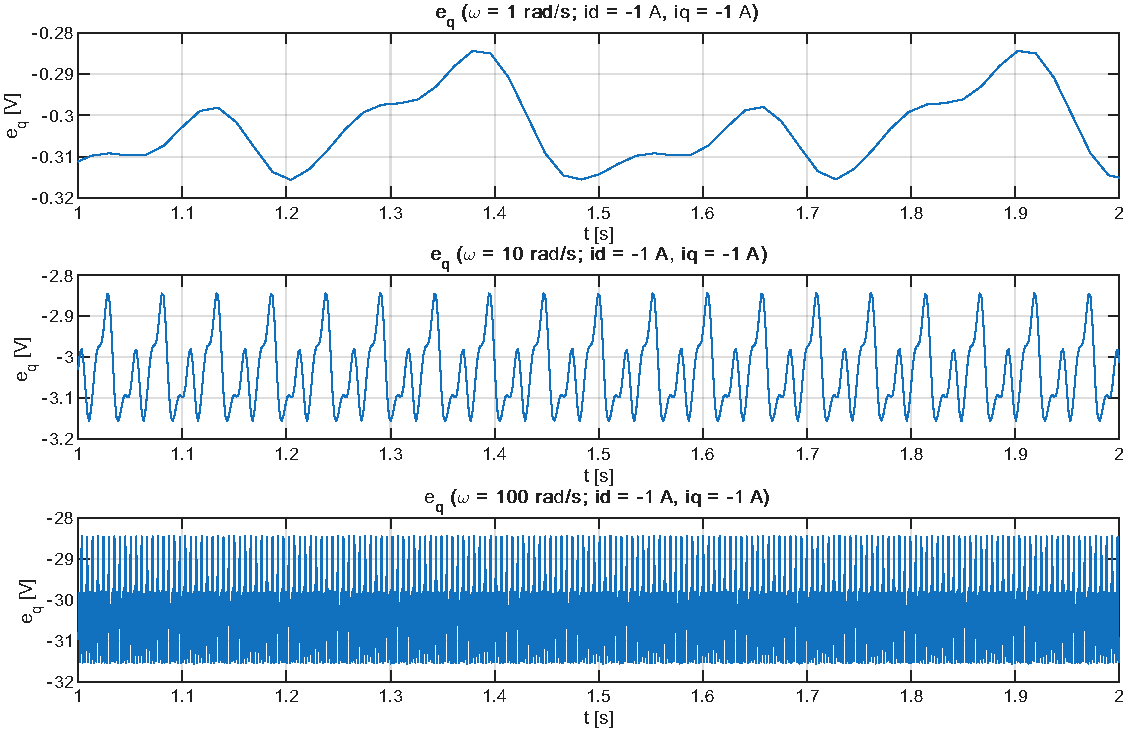
\includegraphics[height=7.5 cm]{immagini/fcem/fcem_Q_vs_velocità.pdf}
    \caption{Andamento della tensione fcem Q al variare della velocità ($i_d$ = -1 A, $i_q$ = 1 A).}
    \label{fig:fcem_Q_vs_velocità}
\end{figure}



\begin{figure}
\centering
    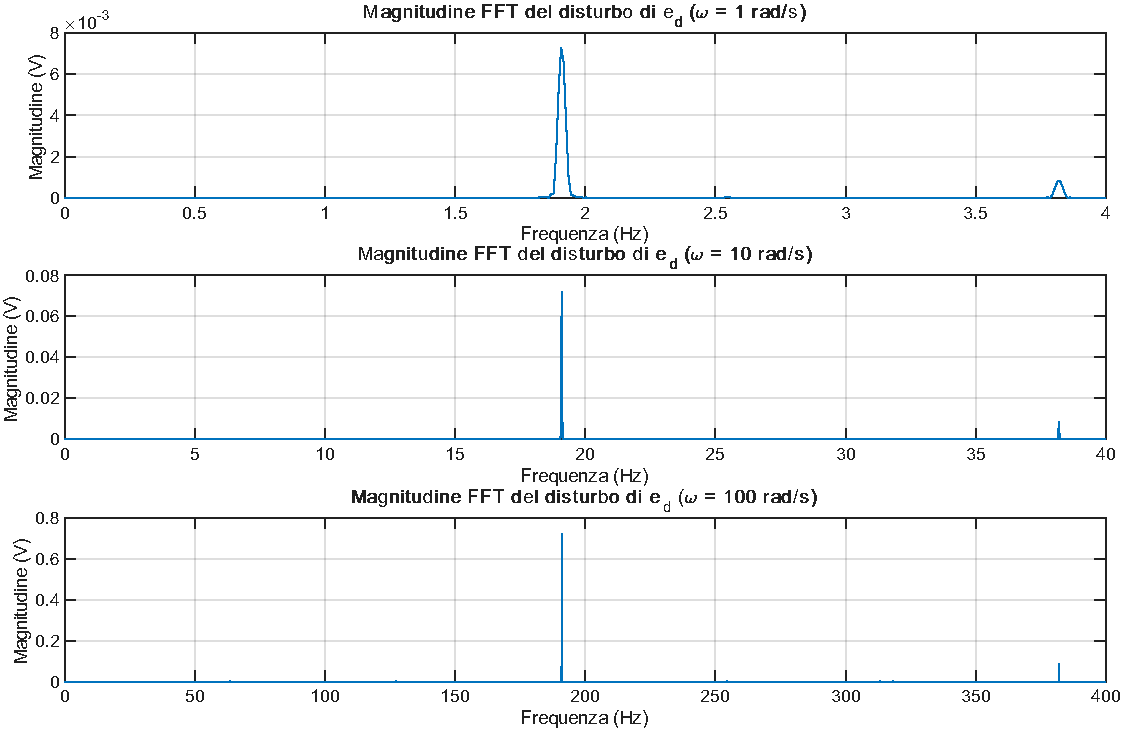
\includegraphics[height=7.5 cm]{immagini/fcem/FFT_fcem_D.pdf}
    \caption{FFT della fcem D al variare della velocità ($i_d$ = $i_q$ = -1 A).}
    \label{fig:FFT_fcem_D}
\end{figure}

\begin{figure}
\centering
    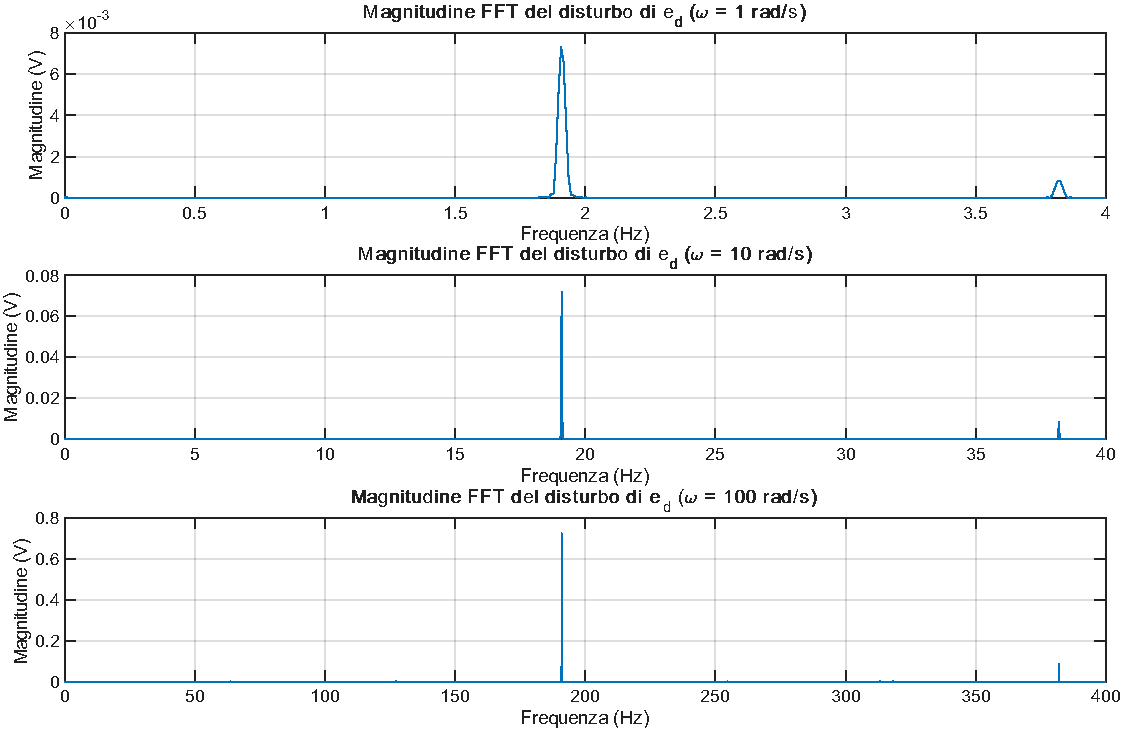
\includegraphics[height=7.5 cm]{immagini/fcem/iq=m1/FFT_fcem_D_iq_1.pdf}
    \caption{FFT della componente d della fcem al variare della velocità ($i_d$ = -1 A, $i_q$ = 1 A).}
    \label{FFT_fcem_D_iq_1}
\end{figure}

\begin{table}
    \centering
        
    \footnotesize
    
    \textbf{Analisi sulla fcem $e_d$}        
    
    \vspace{0.2cm}

    \renewcommand{\arraystretch}{1.3}
    
    \begin{tabular}{
        >{\centering\arraybackslash}m{3 cm}
        >{\centering\arraybackslash}m{2 cm}        
        >{\centering\arraybackslash}m{2.5 cm}
        }
\arrayrulecolor{black}\toprule
        \textbf{Velocità meccanica } &$\mathbf{Ampiezza}$ &$\mathbf{Frequenza}$ \\
       \text{[\,rad/s\,]} &\text{[\,T\,]} &\text{[\,Hz\,]} \\
            \arrayrulecolor{black}\midrule
            \textbf{1} & 0.0073 & 1.9074 \\
            \arrayrulecolor{GRIG}\midrule
            \textbf{10}      & 0.0718 & 19.102 \\
            \arrayrulecolor{GRIG}\midrule
            \textbf{100}      & 0.723 & 190.983 \\
        \arrayrulecolor{black}\bottomrule
    \end{tabular}
    \caption{Analisi sulla fcem $e_d$ con $i_d\ = \ -1\ A$ e $i_q\ = \ 1\ A$.}
    \label{tab:valore_forme_d'onda_fcem_D}  
\end{table}


La distribuzione in frequenza della fcem rispecchia la distribuzione trovata per la FFT di $\lambda_d$ e $\lambda_q$.



\begin{table}
    \centering
        
    \footnotesize
    
    \textbf{Analisi sulla fcem $e_q$}       
    
    \vspace{0.2cm}

    \renewcommand{\arraystretch}{1.3}
    
    \begin{tabular}{
        >{\centering\arraybackslash}m{3 cm}
        >{\centering\arraybackslash}m{2 cm}        
        >{\centering\arraybackslash}m{2.5 cm}
        }
\arrayrulecolor{black}\toprule
        \textbf{Velocità meccanica } &$\mathbf{Ampiezza}$ &$\mathbf{Frequenza}$ \\
       \text{[\,rad/s\,]} &\text{[\,T\,]} &\text{[\,Hz\,]} \\
            \arrayrulecolor{black}\midrule
            \textbf{1} & 0.009 & 3.8147 \\
            \arrayrulecolor{GRIG}\midrule
            \textbf{10} &   0.0911  & 38.195 \\
            \arrayrulecolor{GRIG}\midrule
            \textbf{100}      & 0.9493 & 381.98 \\
        \arrayrulecolor{black}\bottomrule
    \end{tabular}
    \caption{Analisi sulla fcem $e_q$ con $i_d\ = \ -1\ A$ e $i_q\ = \ 1\ A$.}
    \label{tab:valore_forme_d'onda_fcem_Q} 
\end{table}

\section{Stima della curva MTPA}
Si può poi analizzare l'andamento del flusso lungo la curva dei punti MTPA.
Tali punti sono di particolare interesse perchè la curva MTPA comprende tutti quei punti di corrente che sono coinvolti in tale controllo.\\
Per tracciare tale curva, si è eliminata la dipendenza della posizione, mediando per ogni coppia di correnti il flusso magnetico su un giro meccanico. L'obiettivo infatti non è quello di ottenere una stima precisa della curva MTPA, ma un valore indicativo per poi selezionare dei punti di corrente di interesse per l'analisi del flusso magnetico concatenato.\\
Per stimare la curva MTPA si utilizza una funzione di minimizzazione. \\
L'obiettivo è quello di ottenere a parità di corrente il valore massimo di coppia erogabile. Per far ciò si definisce come funzione di costo l'espressione della coppia con segno negativo:




\section{Analisi del flusso rispetto al punto nominale}
Si possono calcolare le coordinate del punto nominale della curva considerando il vincolo imposto dalla corrente nominale ($I_N = 4.2\,\mathrm{A}$).
Tale punto è individuato dall'intersezione tra la curva MTPA e la circonferenza di corrente avente come raggio la corrente nominale.
Si ottiene che le componenti di corrente nominale sono $i_d = -2.769$ A e $i_q = 3.158$ A. Il vincolo sulla corrente è rappresentato visivamente in Figura \ref{fig:Risultati_MTPA}.\\
Il profilo del flusso magnetico associato al punto di corrente nominale è riportato in Figura \ref{fig:Confronto_Flussi_PuntoTarget_0}
Al contrario del caso precedente, si nota una riduzione dell'ampiezza dell'oscillazione sul flusso all'aumentare della corrente.

\begin{figure}
\centering
    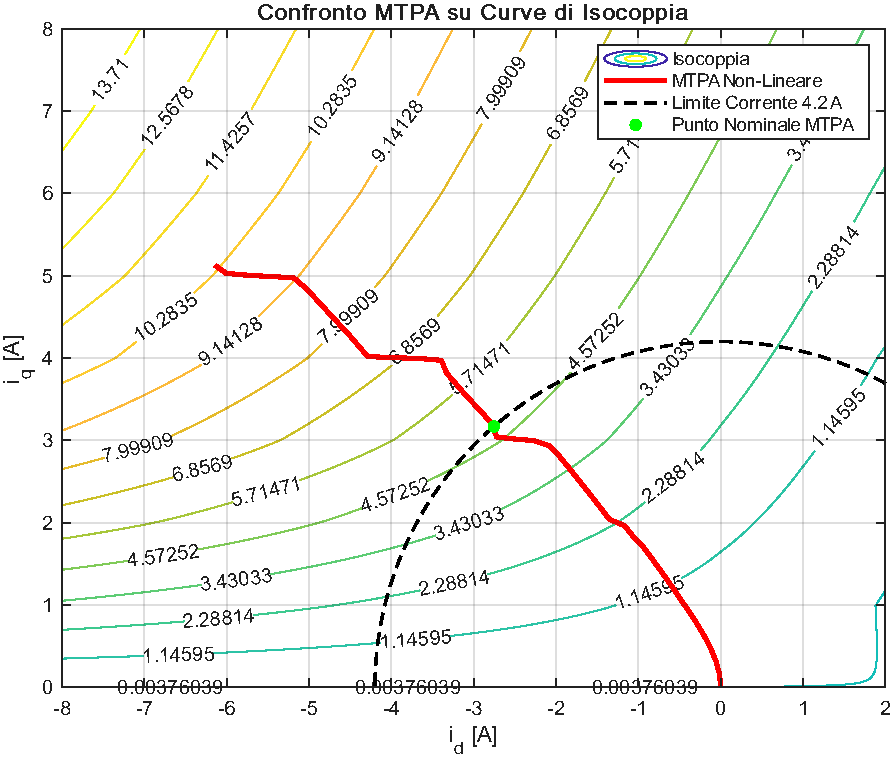
\includegraphics[height=8 cm]{immagini/MTPA/Risultati_MTPA.pdf}
    \caption{Curva MTPA del motore IPM. Il vincolo sulla corrente è rappresentato dall'arco di circonferenza.}
    \label{fig:Risultati_MTPA}
\end{figure}






\subsection{Analisi dell'andamento di $\lambda_{dq}$ al variare della corrente rispetto ai punti della curva MTPA}
Si procede quindi esaminando i grafici del flusso ottenuti muovendosi lungo la curva MTPA, utilizzando $\theta_m$ come parametro. Ciò significa che i flussi $\lambda_d$ e $\lambda_q$ sono stati calcolati rispetto ai punti di corrente lungo la curva.\\
Si può quindi analizzare varia il flusso $\lambda_d$ spostandosi lungo la curva MTPA (Figure \ref{fig:Flusso_D_vs_Id_MTPA_Specifictheta} e \ref{fig:Flusso_D_vs_Iq_MTPA_Specifictheta}).
Allo stesso modo si analizza come varia il valore di $\lambda_q$ spostandosi lungo la curva MTPA (Figure \ref{fig:Flusso_Q_vs_Id_MTPA_Specifictheta} e \ref{fig:Flusso_Q_vs_Iq_MTPA_Specifictheta}).\\
Si procede poi con l'analizzare l'andamento del flusso $\lambda_d$  rispetto alla corrente $i_d$ (Figura \ref{fig:MTPA_Flusso_D_vs_Iq_thetaVar}) e $i_q$ nominale (Figura \ref{fig:MTPA_Flusso_D_vs_Id_thetaVar}), mentre l'altra componente di corrente viene fatta variare.\\
In seguito, si effettua lo stesso tipo di analisi per il flusso $\lambda_q$ (Figura \ref{fig:MTPA_Flusso_Q_vs_Iq_thetaVar} e \ref{fig:MTPA_Flusso_Q_vs_Id_thetaVar}).\\
Il fatto che i grafici presentano delle variazioni nette di pendenza è dovuto all'andamento non lineare della curva MTPA.


\begin{figure}
\centering
    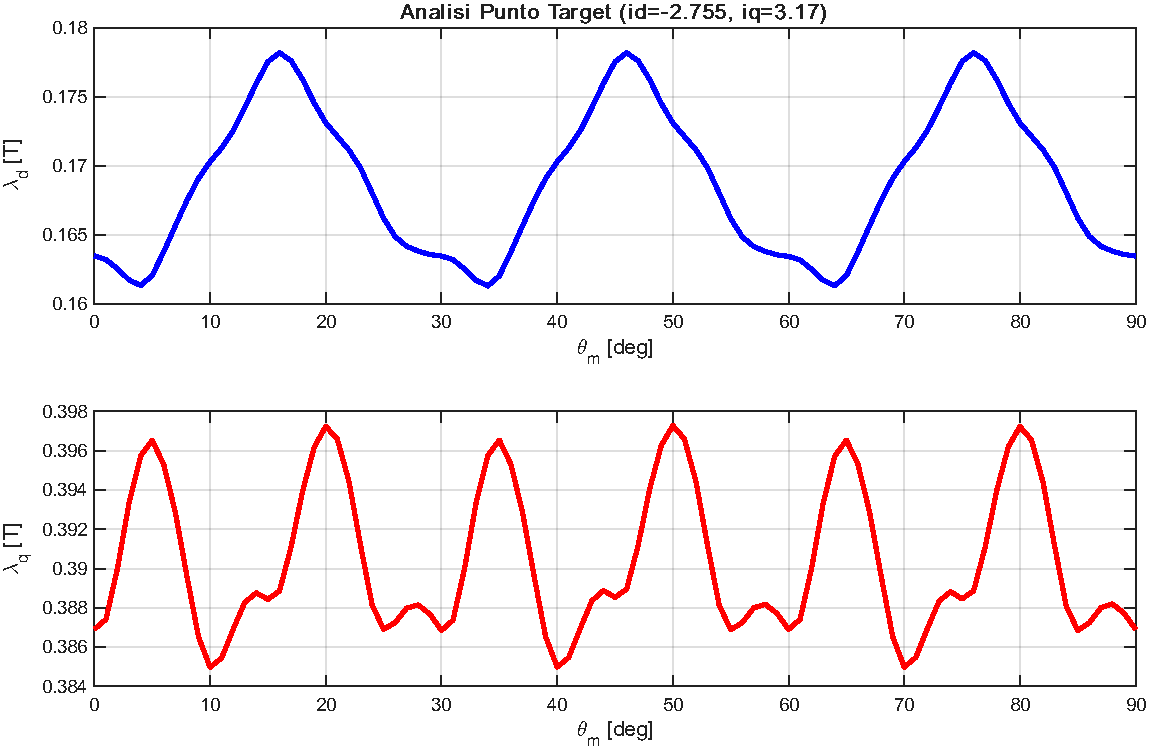
\includegraphics[height=8 cm]{immagini/MTPA/Confronto_Flussi_PuntoTarget_0.pdf}
    \caption{Andamento del flusso D e Q in corrispondenza del punto MTPA nominale a seconda della posizione meccanica $\theta_m$ @ $i_q$ = 3.224 A.}   
    \label{fig:Confronto_Flussi_PuntoTarget_0}
\end{figure}




\begin{figure}
\centering
    \includegraphics[height=8 cm]{immagini/MTPA/Flusso_D_vs_Id_MTPA_Specifictheta.pdf}
    \caption{Andamento di $\lambda_d$ in funzione di $i_d$ a seconda della posizione meccanica $\theta_m$, seguendo la curva MTPA.}    \label{fig:Flusso_D_vs_Id_MTPA_Specifictheta}
\end{figure}

\begin{figure}
\centering
    \includegraphics[height=8 cm]{immagini/MTPA/Flusso_D_vs_Iq_MTPA_Specifictheta.pdf}
    \caption{Andamento di $\lambda_d$ in funzione di $i_q$ a seconda della posizione meccanica $\theta_m$, seguendo la curva MTPA.}   \label{fig:Flusso_D_vs_Iq_MTPA_Specifictheta}
\end{figure}



\begin{figure}
\centering
    \includegraphics[height=8 cm]{immagini/MTPA/Flusso_Q_vs_Id_MTPA_Specifictheta.pdf}
    \caption{Andamento di $\lambda_q$ in funzione di $i_d$ a seconda della posizione meccanica $\theta_m$, seguendo la curva MTPA.}   \label{fig:Flusso_Q_vs_Id_MTPA_Specifictheta}
\end{figure}

\begin{figure}
\centering
    \includegraphics[height=8 cm]{immagini/MTPA/Flusso_Q_vs_Iq_MTPA_Specifictheta.pdf}
    \caption{Andamento di $\lambda_q$ in funzione di $i_q$ a seconda della posizione meccanica $\theta_m$, seguendo la curva MTPA.}   \label{fig:Flusso_Q_vs_Iq_MTPA_Specifictheta}
\end{figure}



\begin{figure}
\centering
    
\includegraphics[height=8 cm]{immagini/MTPA/Flusso_D_vs_Iq_thetaVar.pdf}
    \caption{Andamento del flusso D in funzione di $i_q$ a seconda della posizione meccanica $\theta_m$ @ $i_d$ = -2.755 A.}   
    \label{fig:MTPA_Flusso_D_vs_Iq_thetaVar}
\end{figure}

\begin{figure}
\centering
    
\includegraphics[height=8 cm]{immagini/MTPA/Flusso_D_vs_Id_thetaVar.pdf}
    \caption{Andamento del flusso D in funzione di $i_d$ a seconda della posizione meccanica $\theta_m$ @ $i_q$ = 3.224 A.}   
    \label{fig:MTPA_Flusso_D_vs_Id_thetaVar}
\end{figure}



\begin{figure}
\centering
    
\includegraphics[height=8 cm]{immagini/MTPA/Flusso_Q_vs_Iq_thetaVar.pdf}
    \caption{Andamento del flusso Q in funzione di $i_q$ a seconda della posizione meccanica $\theta_m$ @ $i_d$ = -2.775.}   
    \label{fig:MTPA_Flusso_Q_vs_Iq_thetaVar}
\end{figure}


\begin{figure}
\centering
    
\includegraphics[height=8 cm]{immagini/MTPA/Flusso_Q_vs_Id_thetaVar.pdf}
    \caption{Andamento del flusso Q in funzione di $i_d$ a seconda della posizione meccanica $\theta_m$ @ $i_q$ = 3.17.}   
    \label{fig:MTPA_Flusso_Q_vs_Id_thetaVar}
\end{figure}

\subsection{Analisi dell'andamento di $\lambda_{dq}$ al variare della posizione meccanica rispetto ai punti della curva MTPA}
Si può analizzare l'andamento di $\lambda_d$ e $\lambda_q$ sui punti della curva MTPA (Figure \ref{fig:Flusso_D_vs_theta_MTPA} e \ref{fig:Flusso_Q_vs_theta_MTPA}) al variare della posizione meccanica $\theta_m$. Si osserva anche come l'ampiezza delle oscillazioni aumenta all'aumentare della corrente in modulo.\\
In Figura \ref{fig:Flusso_Q_vs_theta_MTPA} si può osservare in dettaglio l'andamento di $\lambda_d$ e $\lambda_q$ in corrispondenza del punto nominale MTPA.
Successivamente si è valutato la dipendenza dalla posizione della differenza del flusso $\lambda_d$ lungo la curva MTPA e a corrente nulla, per ogni posizione meccanica (Figura \ref{fig:Differenza_Assoluta_Flusso_D_MTPA_Progression}):
\begin{equation}
   \lambda_d^A(i_{dq}) = \lambda_d({i_{dq}})\Big|_{{i_{dq}}\in \text{MTPA}}-\lambda_d(0,0)
\end{equation}
In Figura \ref{fig:Differenza_Flusso_D_MTPA_vs_Zero} si può vedere in dettaglio l'andamento per il punto nominale MTPA.\\
Il flusso può anche essere espresso in maniera relativa, dividendo per il flusso $\lambda_d$ a corrente nulla (Figura \ref{fig:Differenza_Relativa_Flusso_D_MTPA_Progression}):
\begin{equation}
   \lambda_d^{A,rel}(i_{dq}) = \frac{\lambda_d({i_{dq}})\Big|_{{i_{dq}}\in \text{MTPA}}-\lambda_d(0,0)}{\lambda_d(0,0)}
\end{equation}
Si è valutata anche la dipendenza dalla posizione della differenza del flusso $\lambda_1$ nel punto MTPA nominale e a corrente nominale (Figura \ref{fig:Differenza_Assoluta_Flusso_Q_MTPA_Progression}):
\begin{equation}
    \lambda_q^B(i_{dq})=\lambda_q({i_{dq}})\Big|_{{i_{dq}}\in \text{MTPA}}-\lambda_q({i_{dq}})\Big|_{{i_{dq}}\in \text{MTPA,nom}}
\end{equation}
Un'altra valutazione
Si può analizzare inoltre l'incidenza percentuale del ripple di flusso rispetto al  valore medio. I punti di corrente di test appartengono alla curva MTPA.\\
Si analizza poi il profilo del flusso magnetico in funzione della posizione senza la componente media (Figure \ref{fig:Ripple_Relativo_Flusso_D_MTPA} e \ref{fig:Ripple_Relativo_Flusso_Q_MTPA}).\\ In questo modo è possibile esaminare meglio l'impatto della dipendenza della posizione angolare sull'ampiezza di oscillazione.
In Figura \ref{fig:Ripple_Relativo_Flusso_D_MTPA} si può notare come l'ampiezza di oscillazione di $\lambda_d$ relativa aumenti all'aumentare del modulo della corrente. al contrario, l'oscillazione relativa di $\lambda_q$ diminuisce all'aumentare del modulo di corrente (Figura \ref{fig:Ripple_Relativo_Flusso_Q_MTPA}).


\begin{figure}
\centering
    \includegraphics[height=8 cm]{immagini/MTPA/Flusso_D_vs_theta_MTPA.pdf}
    \caption{Andamento del flusso D in funzione della posizione a seconda del punto della curva MTPA analizzato.}
    \label{fig:Flusso_D_vs_theta_MTPA}
\end{figure}

\begin{figure}
\centering
    \includegraphics[height=8 cm]{immagini/MTPA/Flusso_Q_vs_theta_MTPA.pdf}
    \caption{Andamento del flusso Q in funzione della posizione a seconda del punto della curva MTPA analizzato.}
    \label{fig:Flusso_Q_vs_theta_MTPA}
\end{figure}


\begin{figure}
\centering
    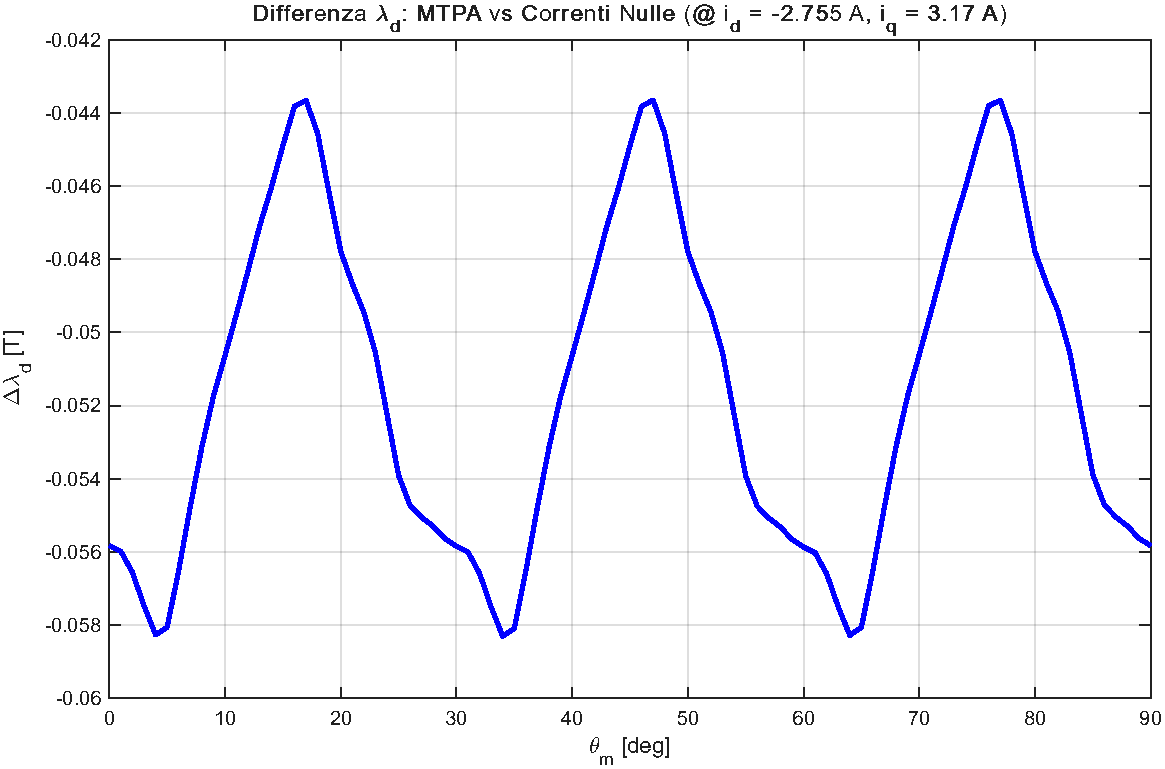
\includegraphics[height=8 cm]{immagini/MTPA/Differenza_Flusso_D_MTPA_vs_Zero.pdf}
    \caption{Differenza del flusso  nel punto MTPA nominale e a corrente nulla, per ogni posizione meccanica, in funzione di $\theta_M$ @ $i_d$ = -2.755, $i_q$ = 3.17 A.} 
    \label{fig:Differenza_Flusso_D_MTPA_vs_Zero}
\end{figure}



\begin{figure}
\centering
    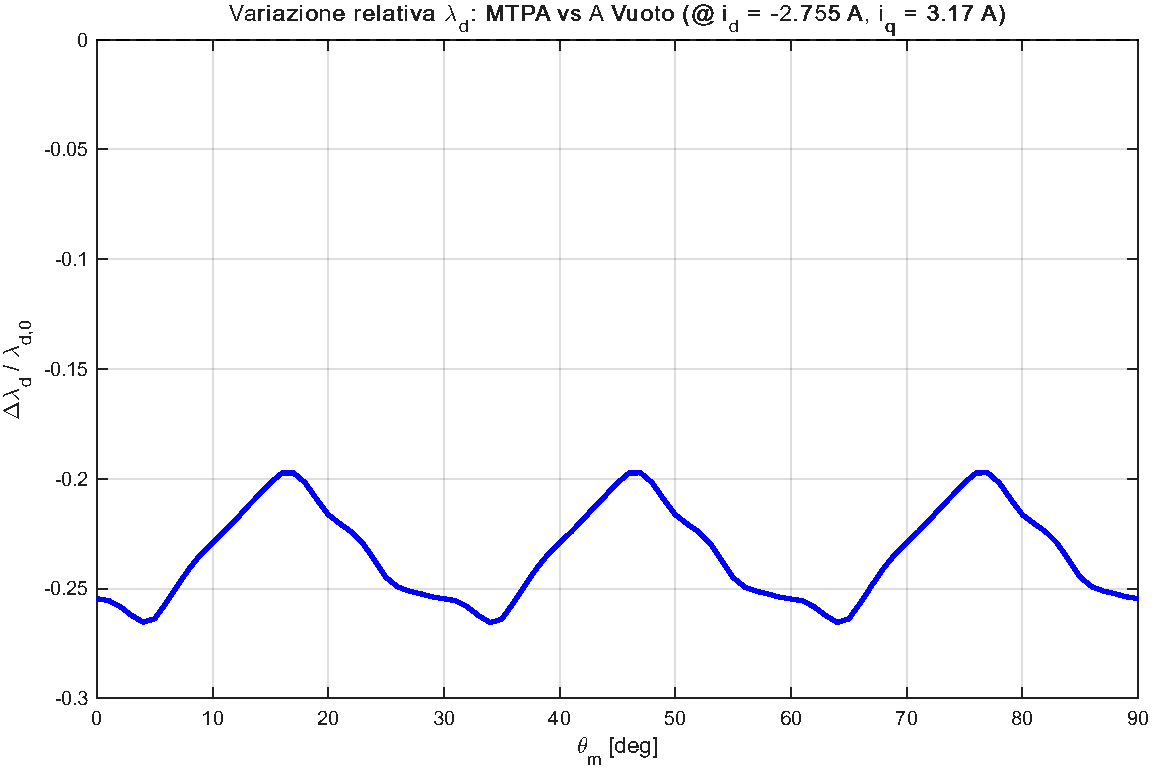
\includegraphics[height=8 cm]{immagini/MTPA/Differenza_Relativa_Flusso_D.pdf}
    \caption{Differenza del flusso  nel punto MTPA nominale e a corrente nulla, normalizzato sul flusso a corrente nulla, in funzione di $\theta_M$, nor @ $i_d$ = -2.755 A, $i_q$ = 3.17 A.} 
    \label{fig:Differenza_Relativa_Flusso_D}
\end{figure}



\begin{figure}
\centering
    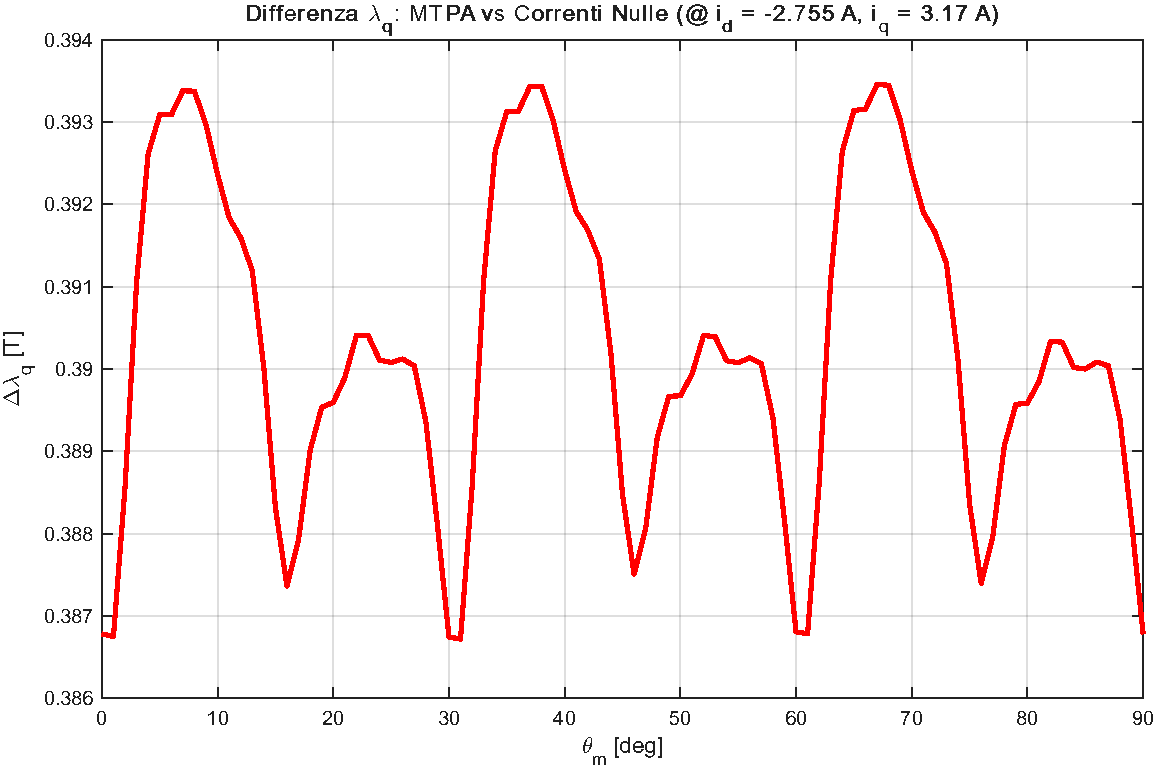
\includegraphics[height=8 cm]{immagini/MTPA/Differenza_Flusso_Q_MTPA_vs_Zero.pdf}
    \caption{Differenza del flusso Q in funzione di $\theta_M$, sottraendo il flusso Q a corrente nulla, @ $i_d$ = -2.755, $i_q$ = 3.17 A.} 
    \label{fig:Differenza_Flusso_Q_MTPA_vs_Zero}
\end{figure}

\begin{figure}
\centering
    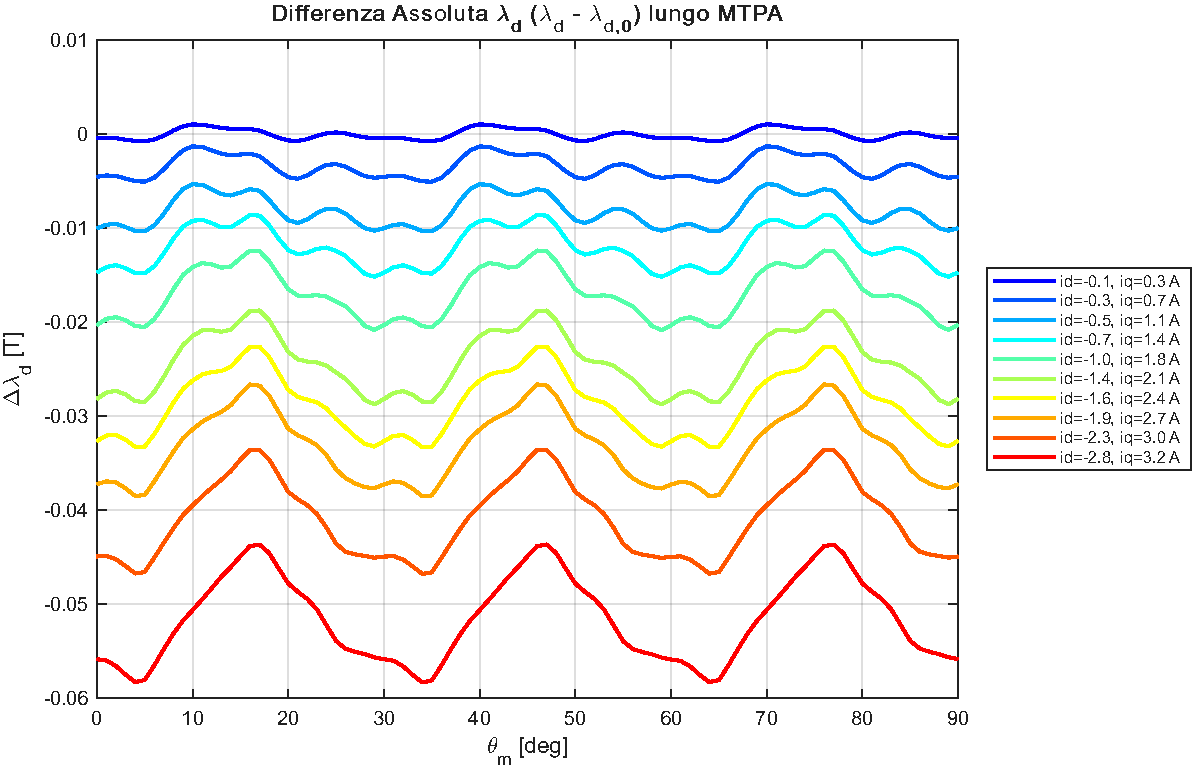
\includegraphics[height=8 cm]{immagini/MTPA/MTPA_multiplo/Differenza_Assoluta_Flusso_D_MTPA_Progression.pdf}
    \caption{Differenza del flusso Q in funzione di $\theta_M$, sottraendo il flusso D a corrente nulla, lungo la curva MTPA.} 
    \label{fig:Differenza_Assoluta_Flusso_D_MTPA_Progression}
\end{figure}

\begin{figure}
\centering
    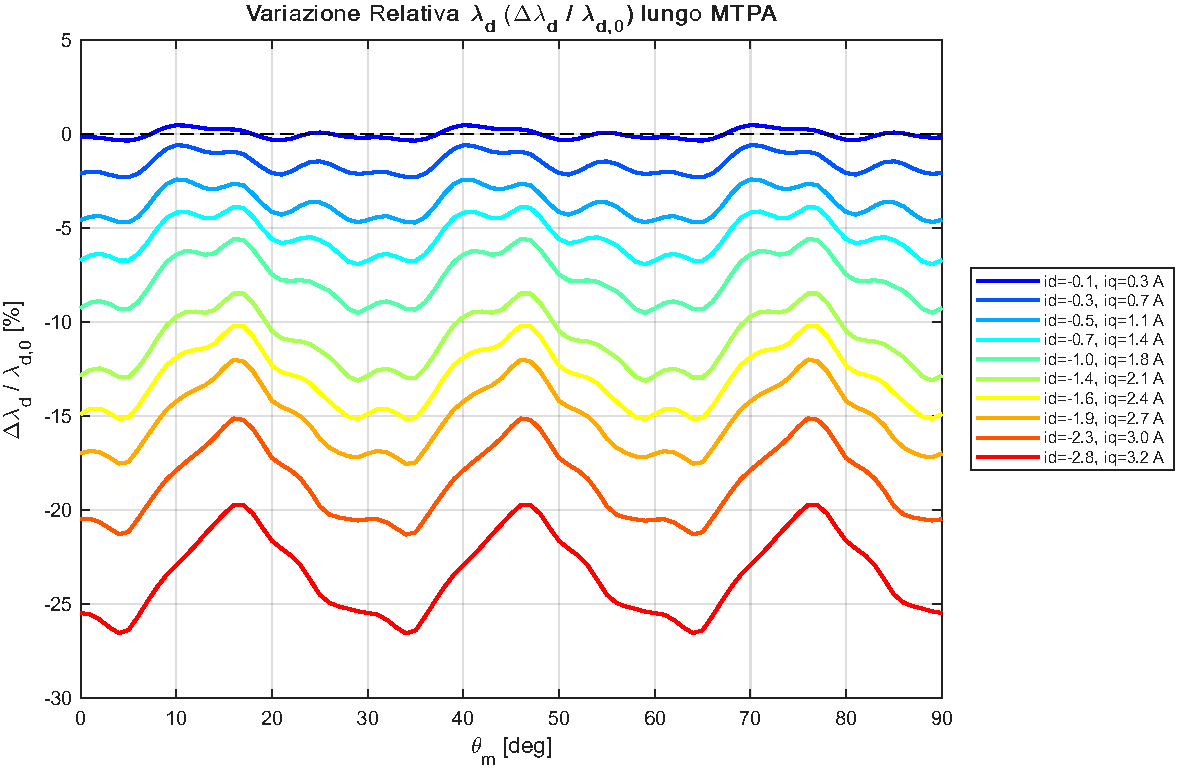
\includegraphics[height=8 cm]{immagini/MTPA/MTPA_multiplo/Differenza_Relativa_Flusso_D_MTPA_Progression.pdf}
    \caption{Differenza del flusso Q in funzione di $\theta_M$, sottraendo il flusso D a corrente nulla e dividendo per esso, lungo la curva MTPA.} 
    \label{fig:Differenza_Relativa_Flusso_D_MTPA_Progression}
\end{figure}


\begin{figure}
\centering
    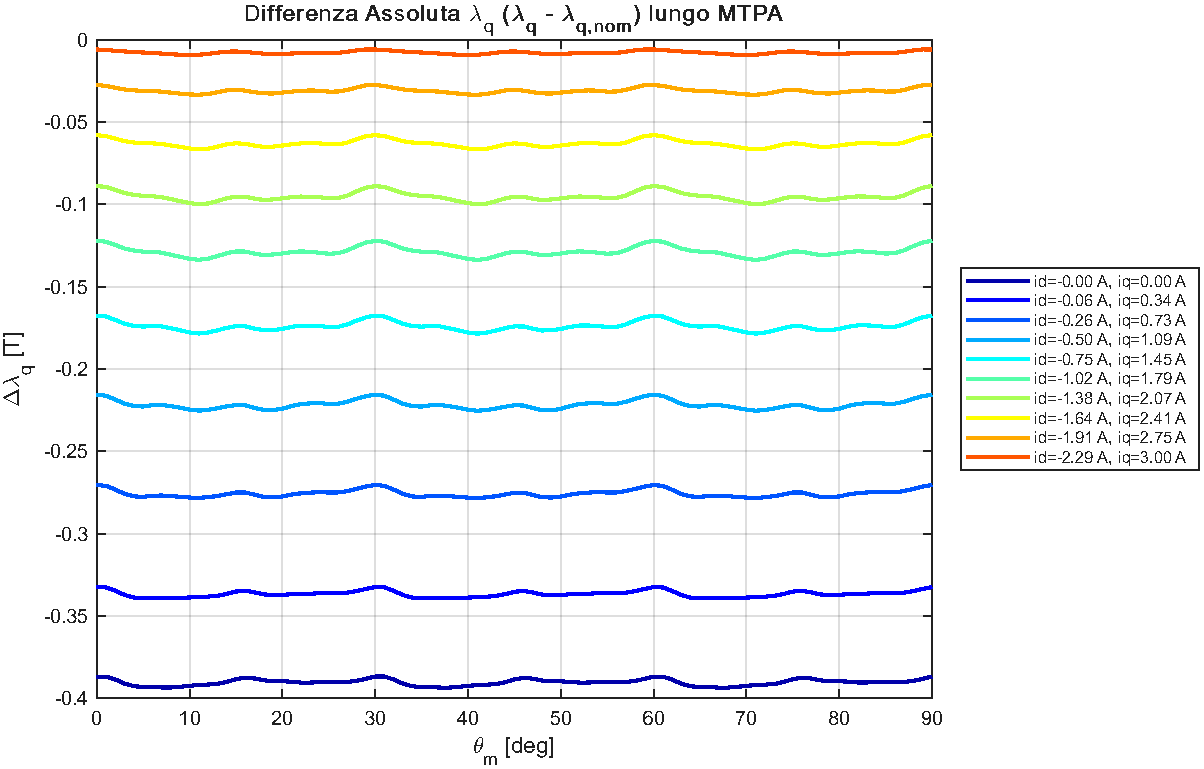
\includegraphics[height=8 cm]{immagini/MTPA/MTPA_multiplo/Differenza_Assoluta_Flusso_Q_MTPA_Progression.pdf}
    \caption{Differenza del flusso Q in funzione di $\theta_M$, sottraendo il flusso D a corrente nominale, lungo la curva MTPA.} 
    \label{fig:Differenza_Assoluta_Flusso_Q_MTPA_Progression}
\end{figure}

\begin{figure}
\centering
    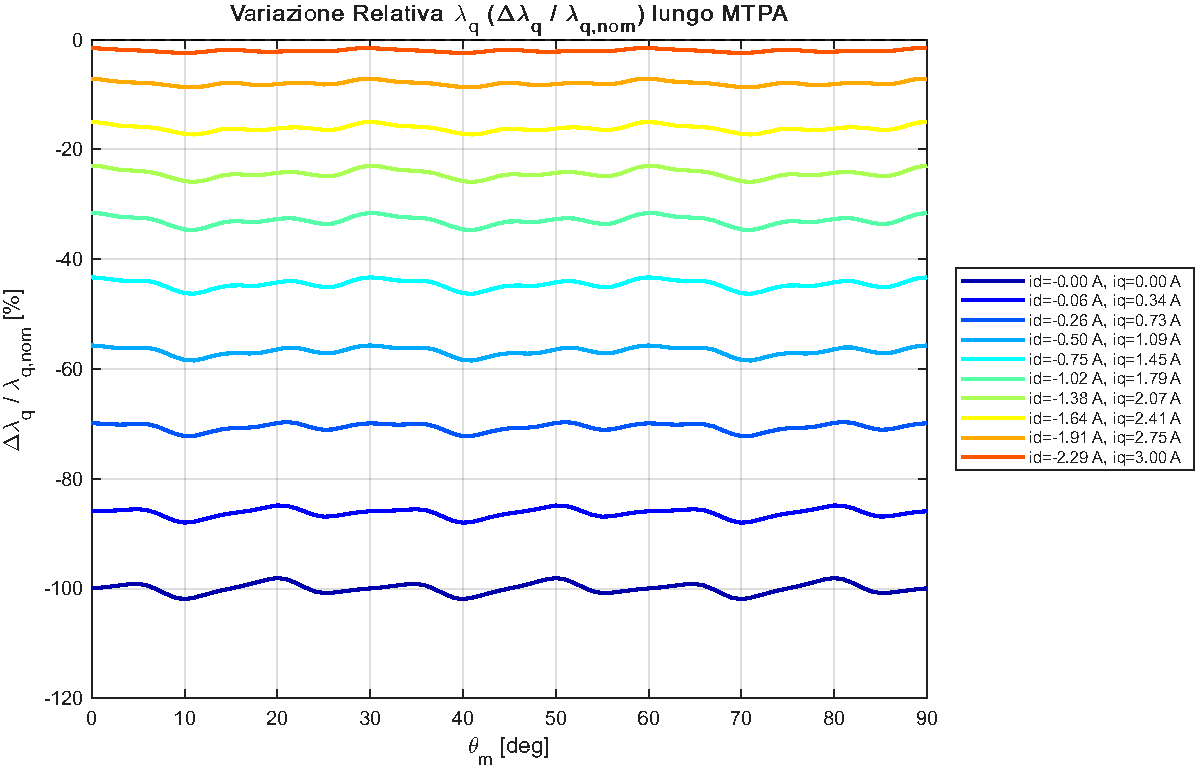
\includegraphics[height=8 cm]{immagini/MTPA/MTPA_multiplo/Differenza_Relativa_Flusso_Q_MTPA_Progression.pdf}
    \caption{Differenza del flusso Q in funzione di $\theta_M$, sottraendo il flusso D a corrente nominale e dividendo per esso, lungo la curva MTPA.} 
    \label{fig:Differenza_Relativa_Flusso_Q_MTPA_Progression}
\end{figure}



\begin{figure}
\centering
    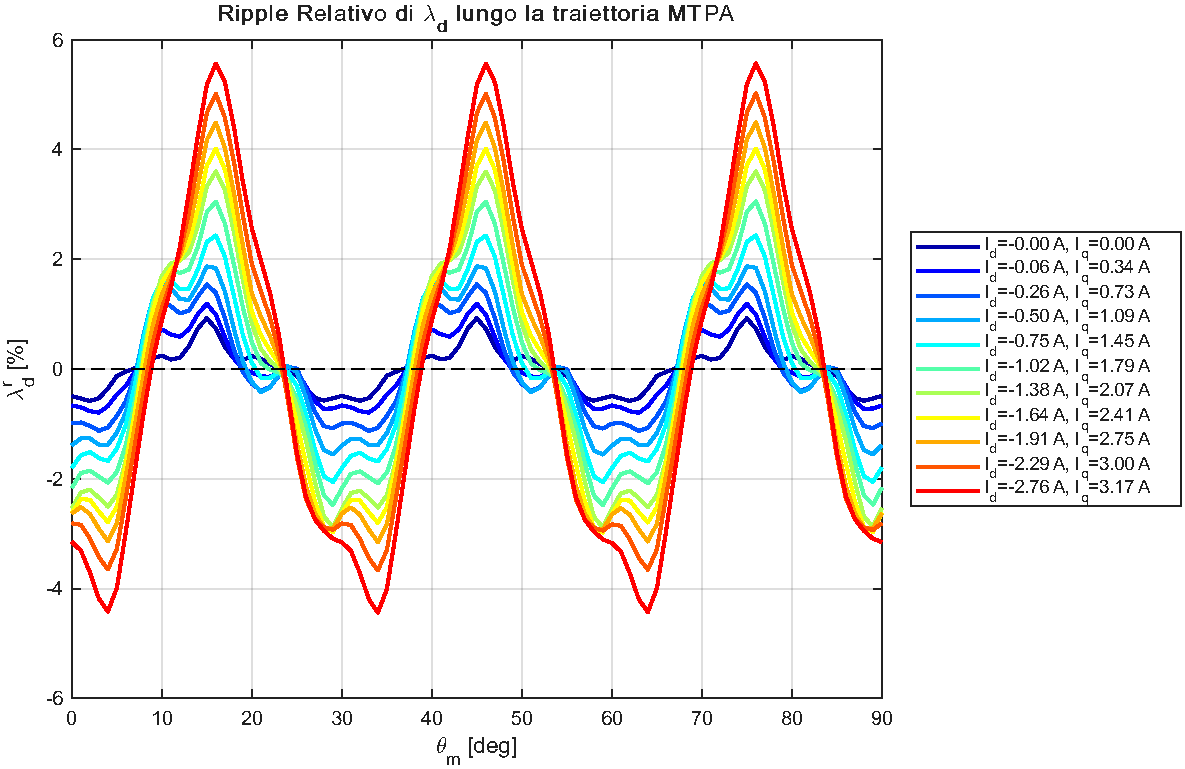
\includegraphics[height=8 cm]{immagini/MTPA/MTPA_multiplo/Ripple_Relativo_Flusso_D_MTPA.pdf}
    \caption{Variazione relativa del flusso D rispetto alla media.} 
    \label{fig:Ripple_Relativo_Flusso_D_MTPA}
\end{figure}



\begin{figure}
\centering
    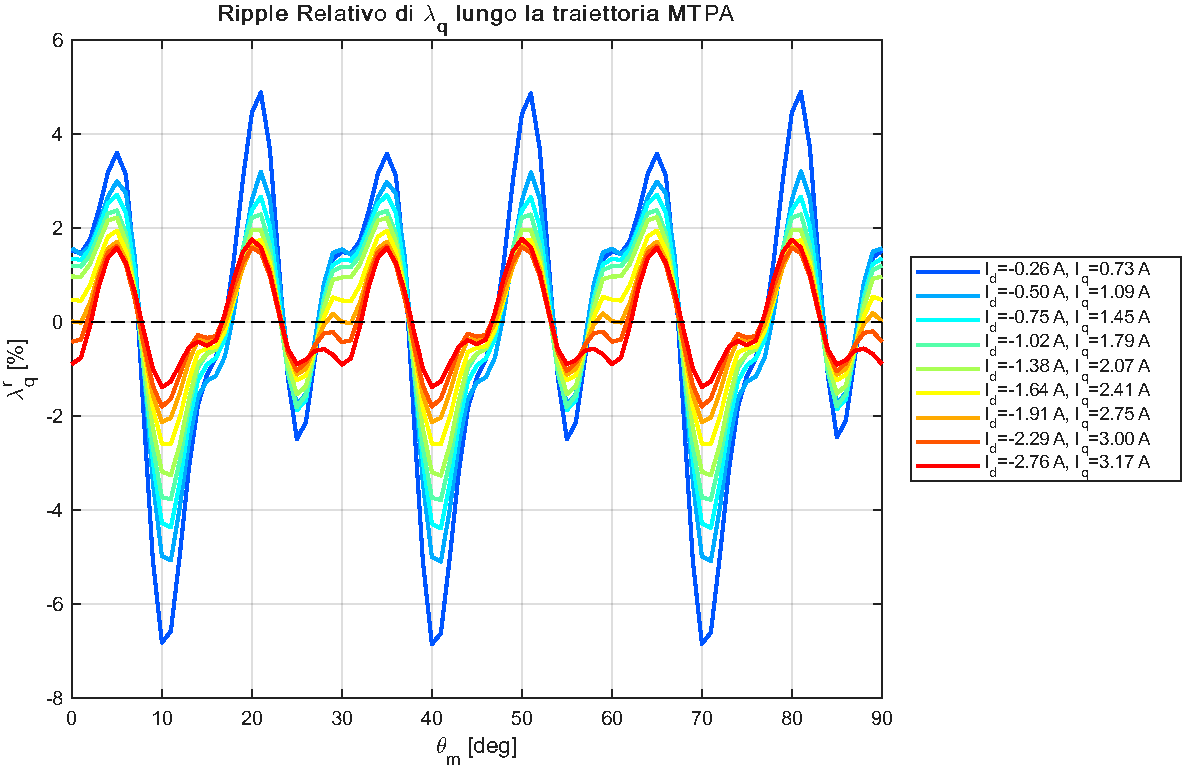
\includegraphics[height=8 cm]{immagini/MTPA/MTPA_multiplo/Ripple_Relativo_Flusso_Q_MTPA.pdf}
    \caption{Variazione relativa del flusso Q rispetto alla media.} 
    \label{fig:Ripple_Relativo_Flusso_Q_MTPA}
\end{figure}